\section{Client}
\label{chapter:client}

Cette section est entièrement dédiée à la conception du \gls{frontend} de \texttt{SourceCode}. Étant donné qu'il s'agit de la partie visuelle et ergonomique du site, nous aborderons cette thématique de manière plus illustrative.\\

Pour ce faire, nous allons naviguer à travers les différentes pages de la plateforme en expliquant nos choix d'implémentation et les fonctionnalités qui ont été mises en place.\\

Afin de vous donner une idée plus claire de ce qui va être abordé, voici une représentation du groupe d'URL de premier niveau que contient \texttt{SourceCode}.\\

\begin{figure}[H]
    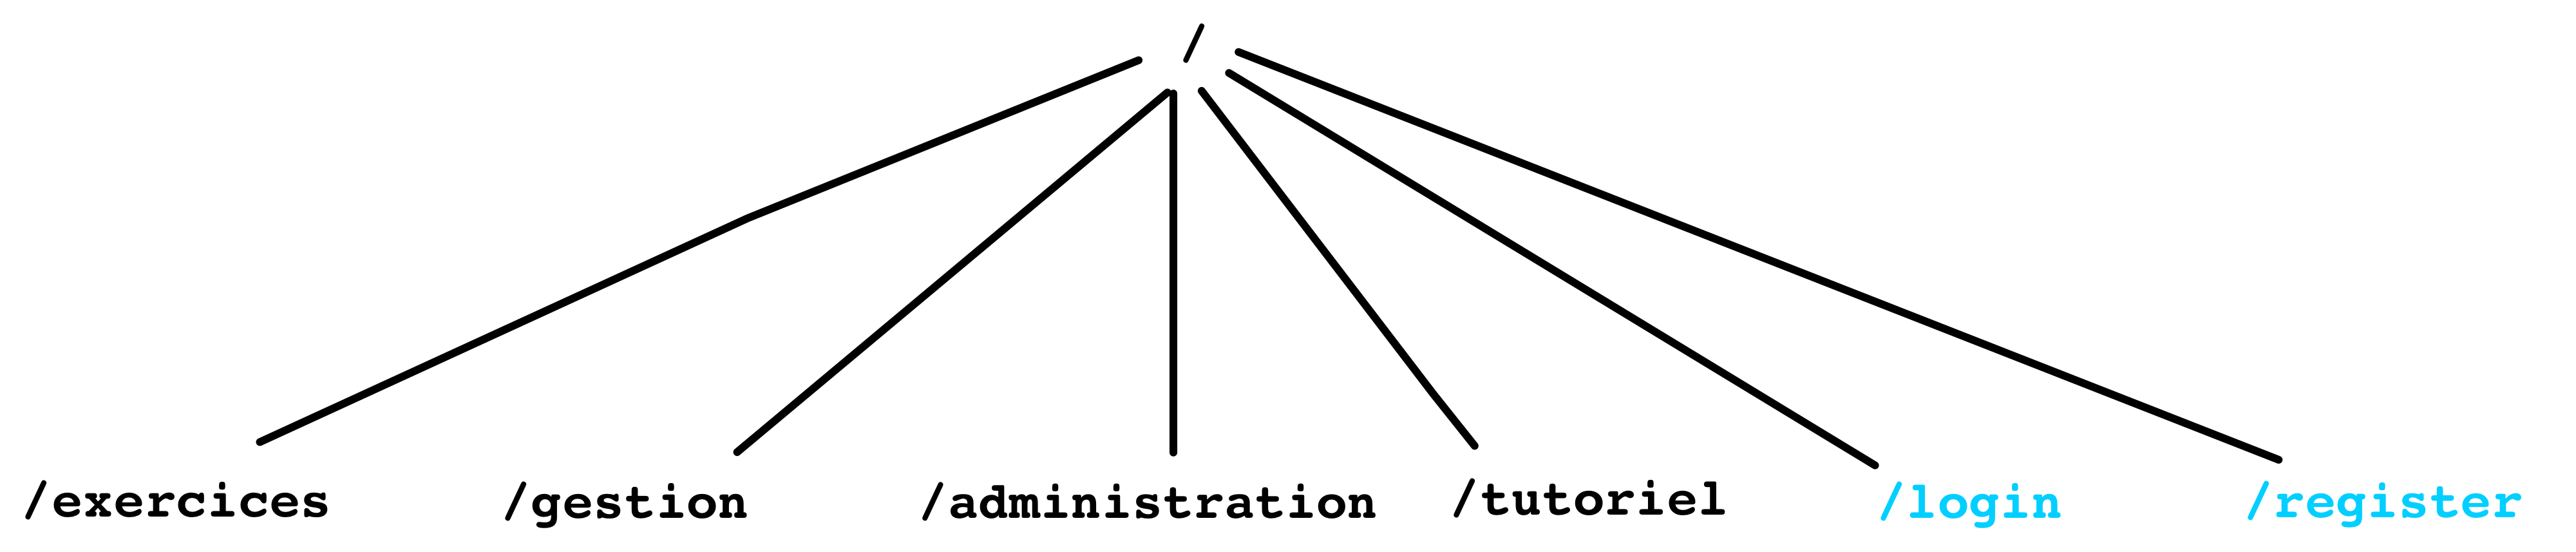
\includegraphics[width=\textwidth,height=0.15\textheight,keepaspectratio]{images/client/overview_client.jpeg}
    \centering
    \caption[SourceCode : Représentation des URL de premier niveau]{URL de premier niveau}
\end{figure}

Cette figure sera notre fil conducteur tout au long de cette section, car nous allons analyser chaque partie en profondeur. 
Les URL en \textbf{noir} signifient qu'elles renferment un niveau supplémentaire d'URL tandis que les \textbf{bleus} désignent une page de contenu.\\

Les deux premières URL de la figure désignent les interfaces de connexion à \texttt{SourceCode} ainsi que la création d'un compte.\\

L'URL \textit{/exercices} représente la bibliothèque de \glspl{resinfo}. C'est dans cet espace que le coeur de \texttt{SourceCode} réside, car c'est là que le système de recherche a été pensé pour tout le reste de la plateforme. En outre,
cette même URL contient aussi la consultation de \glspl{fiche} lorsque les critères de recherche de l'utilisateur sont satisfaits. À noter que tout type d'utilisateur peut accéder à ces pages.\\

L'URL \textit{/gestion} renferme tout ce dont un utilisateur (connecté avec son compte) peut effectuer sur la plateforme pour enrichir son utilisation. On y répertorie la gestion/création/modification de ses propres \glspl{resinfo}, la gestion/création/modification de ses favoris pour faciliter la recherche et enfin, la consultation de son profil. Cette partie est accessible aux utilisateurs et (super-)administrateurs.\\

L'URL \textit{/administration} contient les fonctionnalités exigeant le plus haut niveau de privilèges sur \texttt{SourceCode}. Cette partie est donc entièrement dédiée aux administrateurs et super-administrateurs. Ils peuvent gérer absolument toutes les \glspl{resinfo} disponibles sur la plateforme (impliquant aussi la modification et création de celles-ci), l'importation/exportation de \glspl{resinfo}, la gestion/création/modification de \glspl{tag}, la gestion/création/modification des \glspl{tagCat} et finalement la gestion des utilisateurs de la plateforme.\\

L'URL \textit{/tutoriel} concerne un aspect plus ludique de \texttt{SourceCode}. À travers différentes pages, une thématique de l'application est décortiquée afin que l'utilisateur puisse améliorer sa prise en main avec la plateforme.\\

Avant d'aller plus loin, considérez la section \ref{section:challengesToDefeat} afin de vous remettre en tête ce que nous voulions apporter à \texttt{SourceCode}.

\subsection{Connexion et création de comptes}

La création d'un compte permet d'accéder à des fonctionnalités supplémentaires comme la création de favoris ou de \glspl{resinfo}.\\

\begin{figure}[H]
    
\includegraphics[width=\textwidth,height=0.35\textheight,keepaspectratio]{images/client/register.png}
    \centering
    \caption[SourceCode : interface de création de comptes]{Interface de création de comptes}
\end{figure}

Par défaut, un compte créé offre les privilèges d'un \textbf{utilisateur}. Voici pour rappel (section \ref{section:analyseFonctionnelle}) les différents types d'utilisateurs pouvant accéder à la plateforme :

\begin{itemize}
    \item \textbf{Visiteur} : C'est la forme la plus simple. Les droits de ce type d'utilisateur se limitent à la navigation dans la bibliothèque de \glspl{resinfo}. Le système de favoris n'est accessible qu'à partir du moment où vous êtes membre de la plateforme. Nous entendons par là l'utilisateur ou l'administrateur.
    \item \textbf{Utilisateur} : L'utilisateur est membre de l'application. Il possède donc un compte et peut participer au partage de \glspl{resinfo}. L'utilisateur a la possibilité de créer des favoris qu'il pourra ainsi utiliser dans la bibliothèque ou depuis ses interfaces de gestion.
    \item \textbf{(Super-)administrateur} : L'administrateur est un rôle capital, car lui seul permet de garantir du contenu de qualité. Il est chargé de valider les \glspl{resinfo} soumises par les utilisateurs, de valider les \glspl{tag} et de créer de nouvelles \glspl{tagCat}. En plus de ces droits-ci, l'administrateur possède bien évidemment tous les droits de l'utilisateur !
\end{itemize}

Le formulaire de création nécessite une adresse email (unique), un mot de passe et un nom complet.


\begin{figure}[H]
    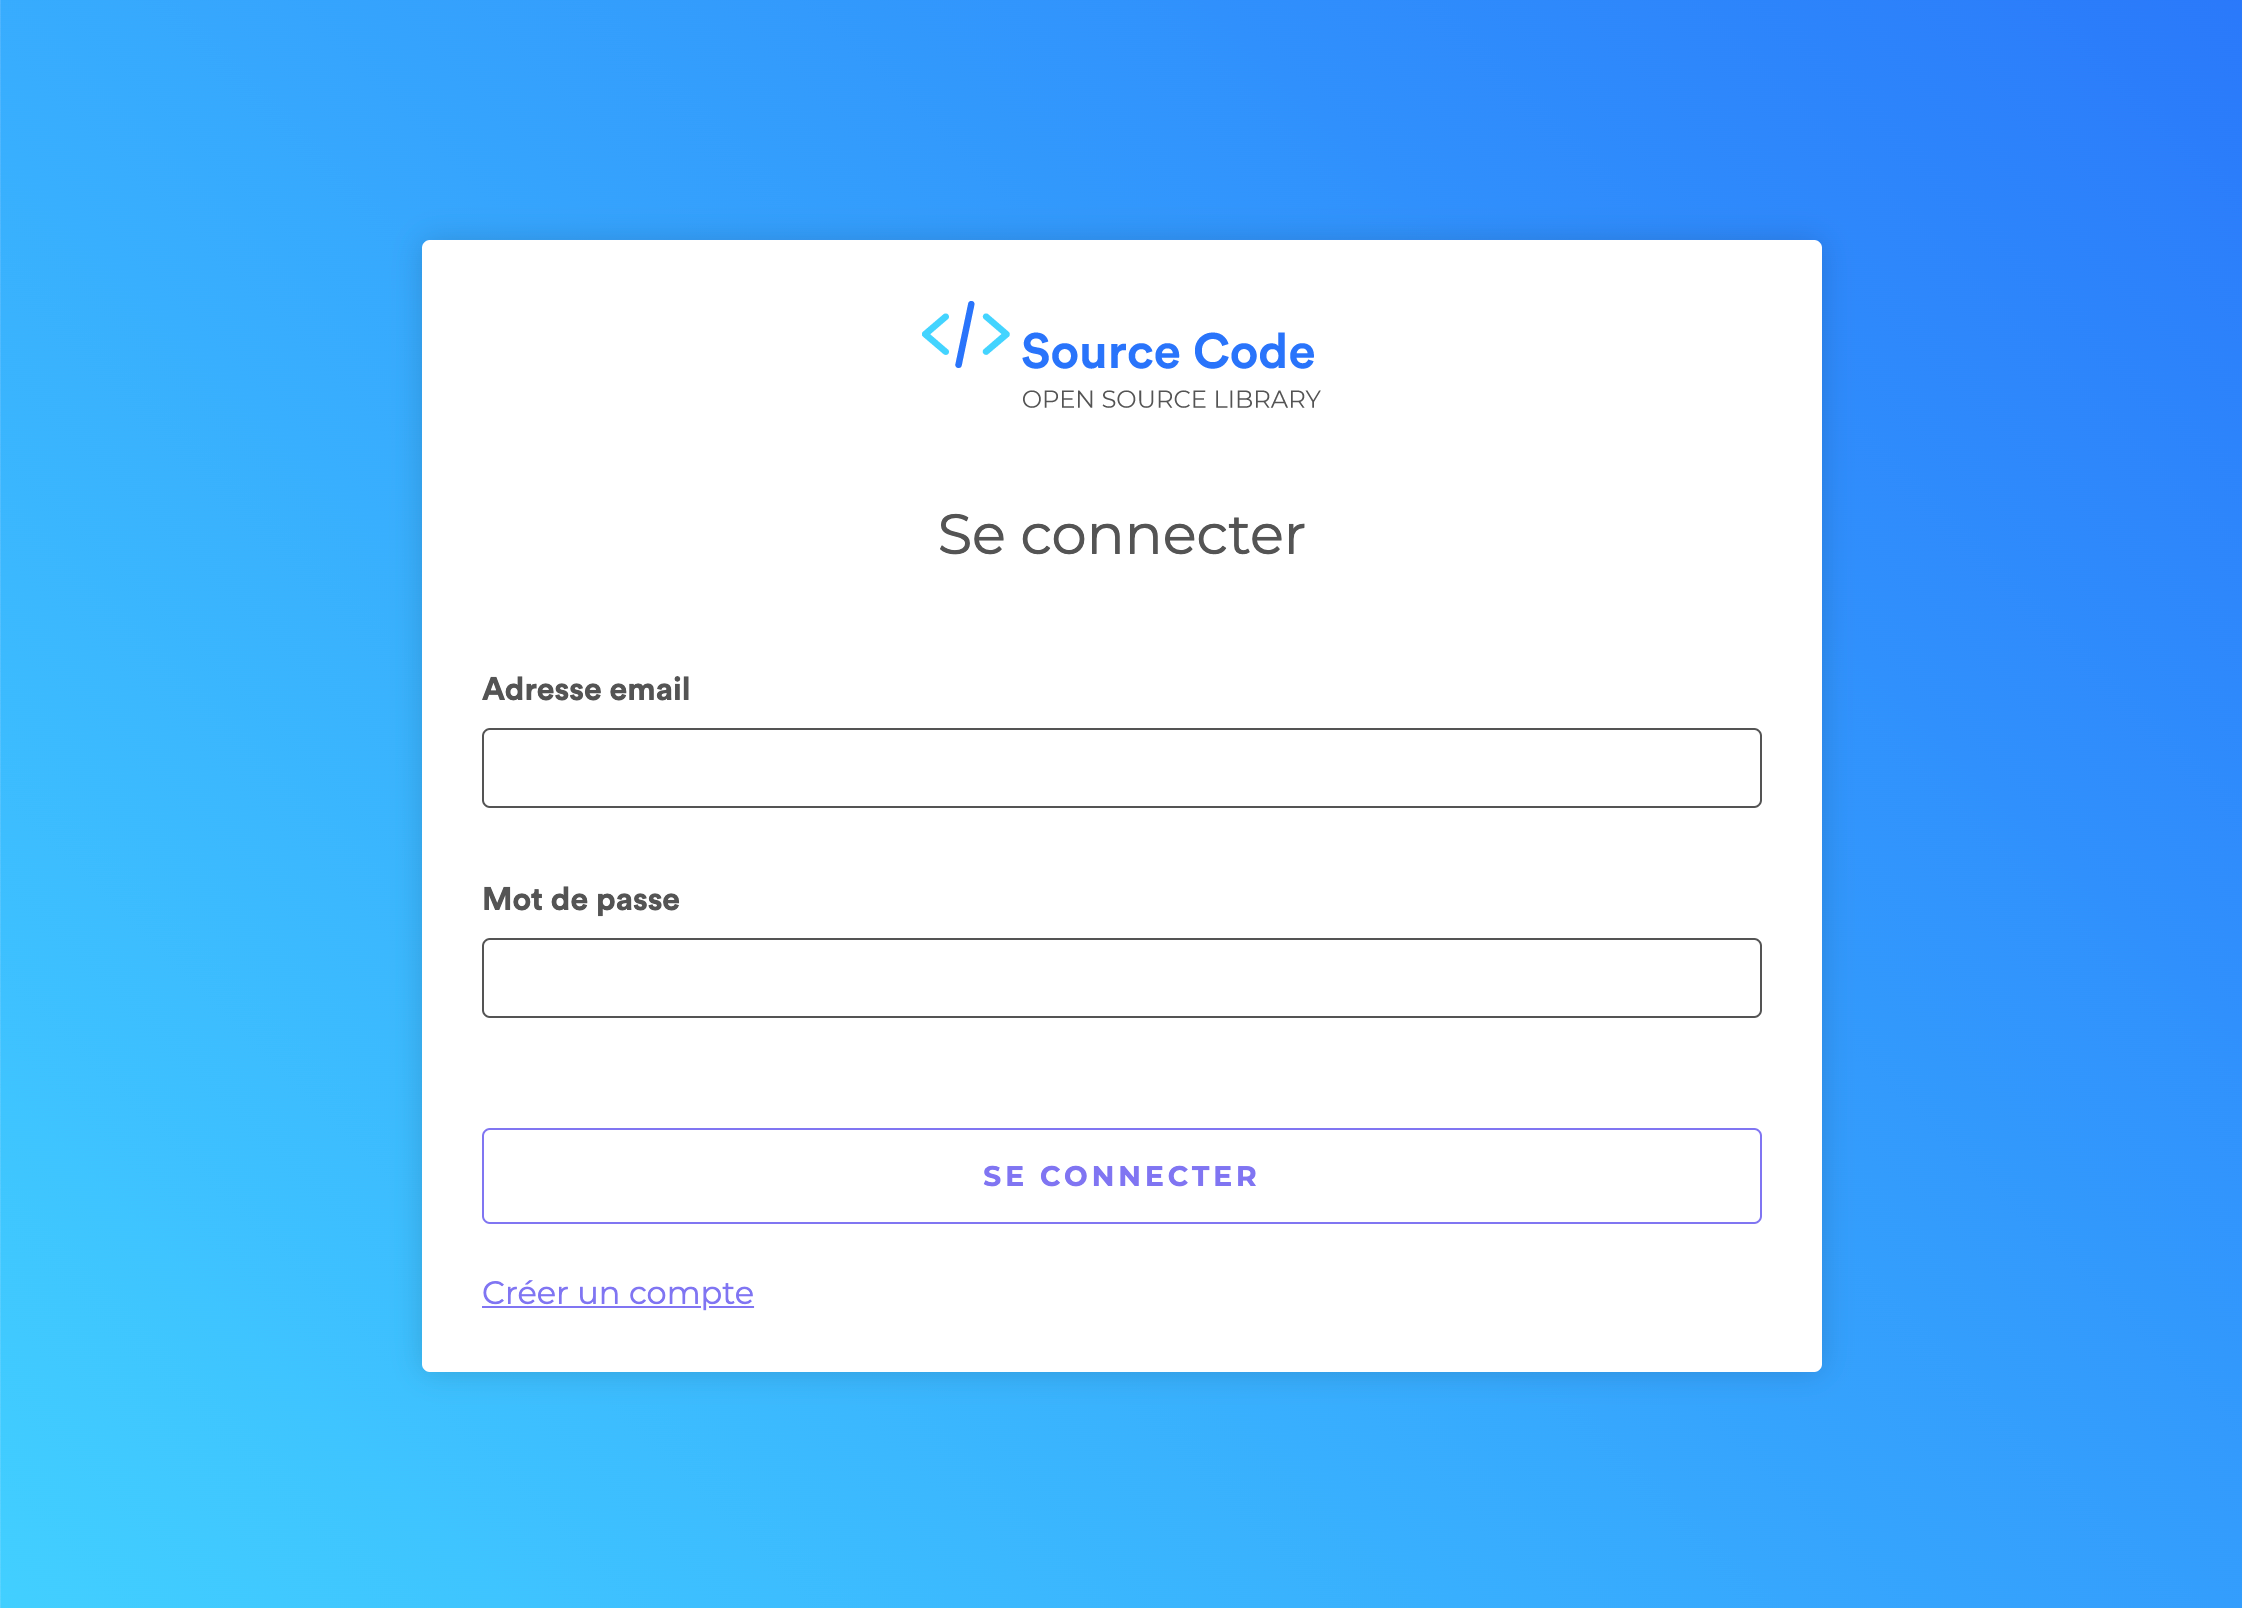
\includegraphics[width=\textwidth,height=0.35\textheight,keepaspectratio]{images/client/login.png}
    \centering
    \caption[SourceCode : interface de connexion]{Interface de connexion}
\end{figure}

Lorsque l'utilisateur possède déjà un compte, il lui suffit de renseigner son adresse email et son mot de passe. Pour l'instant, une session d'une heure lui sera attribuée pour gérer ses ressources, favoris, ... Après quoi il sera redirigé vers la page de login pour entrer à nouveau ses identifiants. Ce comportement est bien évidemment modifiable depuis l'api (cf. section \ref{section:apiConfig}), mais nous avions surtout choisi ce timing pour la séance de validation de notre plateforme (cf. \ref{annexe:googleForm}).\\


\subsection{Exercices}

La bibliothèque constitue l'élément central de \texttt{SourceCode} pour le partage de ressources. C'est dans cet espace que les \glspl{resinfo} validées par la communauté apparaitront.\\

\begin{figure}[H]
    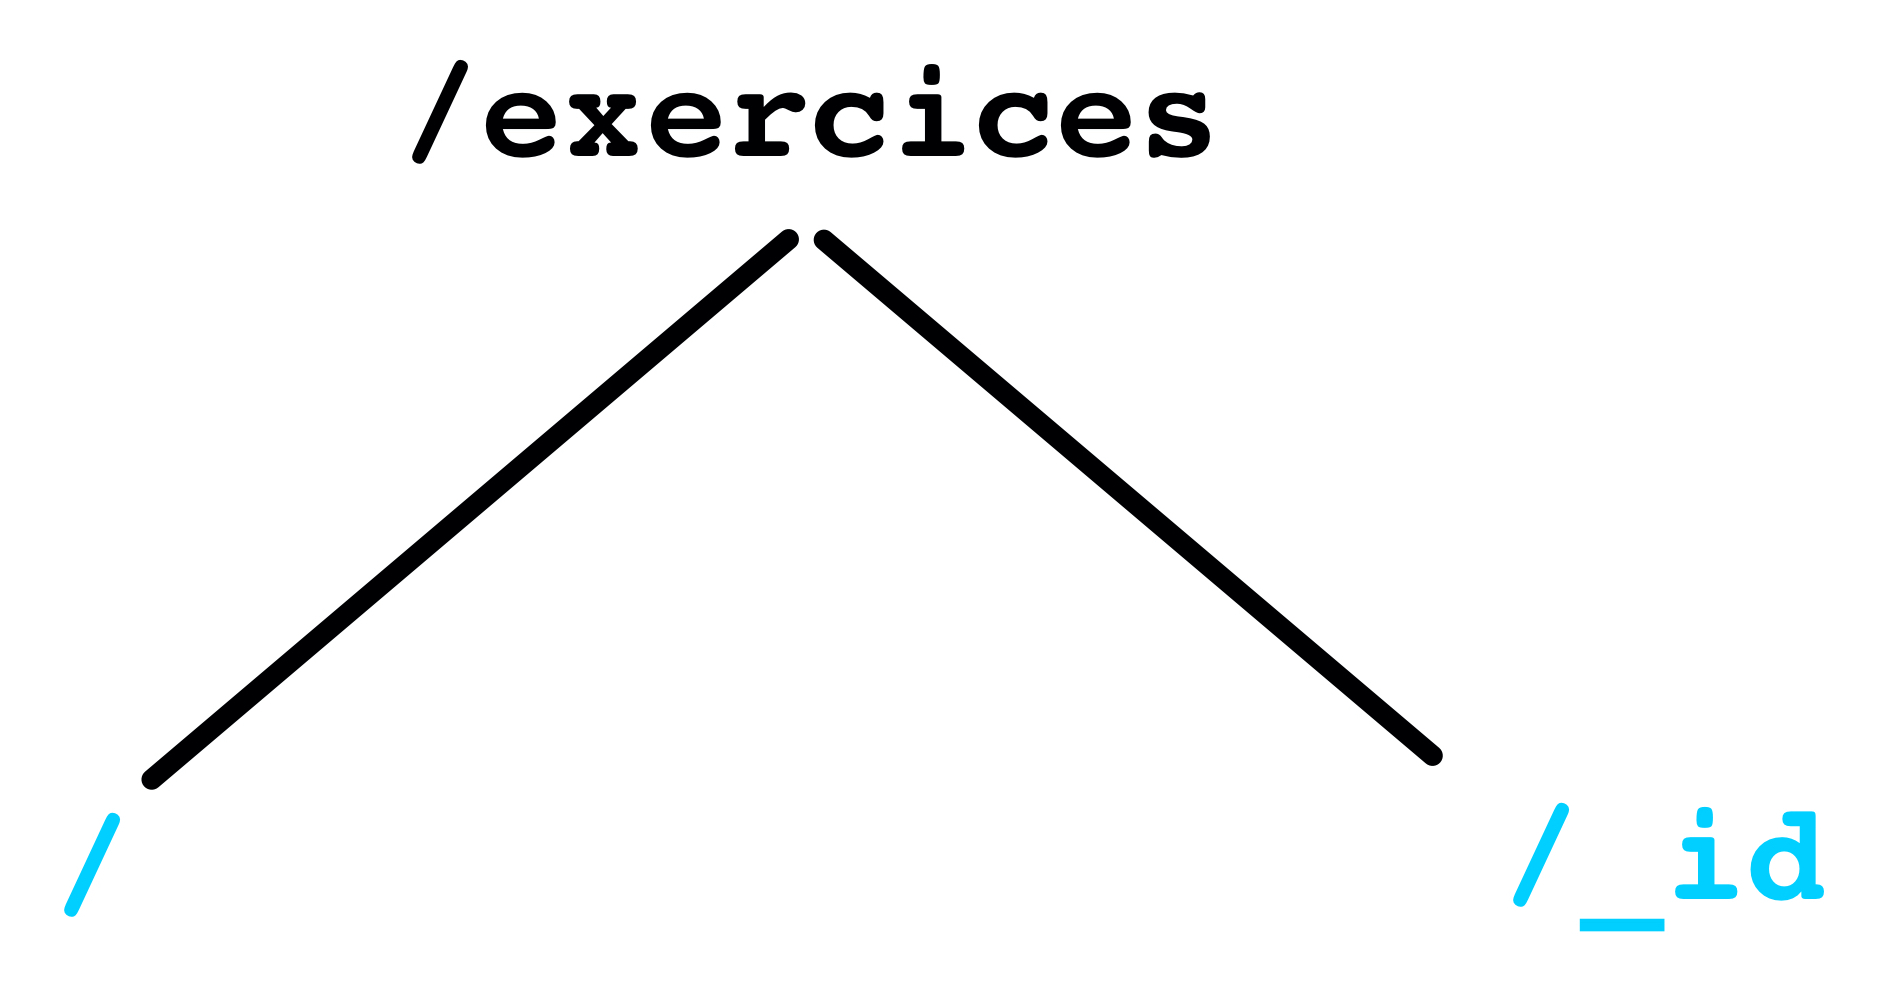
\includegraphics[width=\textwidth,height=0.08\textheight,keepaspectratio]{images/client/exercices.jpeg}
    \centering
    \caption[SourceCode : partie bibliothèque]{Partie bibliothèque (URL)}
\end{figure}

Cette section peut se découper en deux parties distinctes :

\begin{itemize}
    \item La bibliothèque (accessible depuis l'URL \textit{/exercices}) : nous y aborderons le système de recherche mis en place, les privilèges utilisateurs sur cette page ainsi que les choix ergonomiques.\\
    \item La \gls{fiche} d'une \gls{resinfo} (accessible depuis l'URL \textit{/exercices/\_id}\footnote{
        Lorsqu'une URL contient \textit{\_id}, cela peut être remplacé par un nombre naturel $ n $  $\epsilon$   $\mathbb{N}$ $/ \{0\}$. Les id's représentent l'id d'une entité stockée dans la base de données. Exemple : pour récupérer l'exercice ayant l'id 42 (pour autant qu'il existe), il suffit de renseigner l'URL \textit{/exercices/42}.
    }) : nous y expliquerons le référencement de la \gls{fiche} afin d'établir un lien avec de la bibliothèque.
\end{itemize}

\subsubsection{La bibliothèque}

La page \textit{bibliothèque} contient toutes les \glspl{resinfo} ajoutées par la communauté et ayant été validées par les administrateurs de la plateforme. Elle est accessible publiquement, pour tout type d'utilisateurs.\\

Concernant l'interface, nous nous sommes inspirés de \textit{Coderbyte} et \textit{Hackerrank} pour le panneau de filtres et le preview des \glspl{resinfo} (voir section \ref{section:situation}). Il était important pour nous de conserver une interface simple et déjà utilisée par certaines applications web.

\begin{figure}[H]
    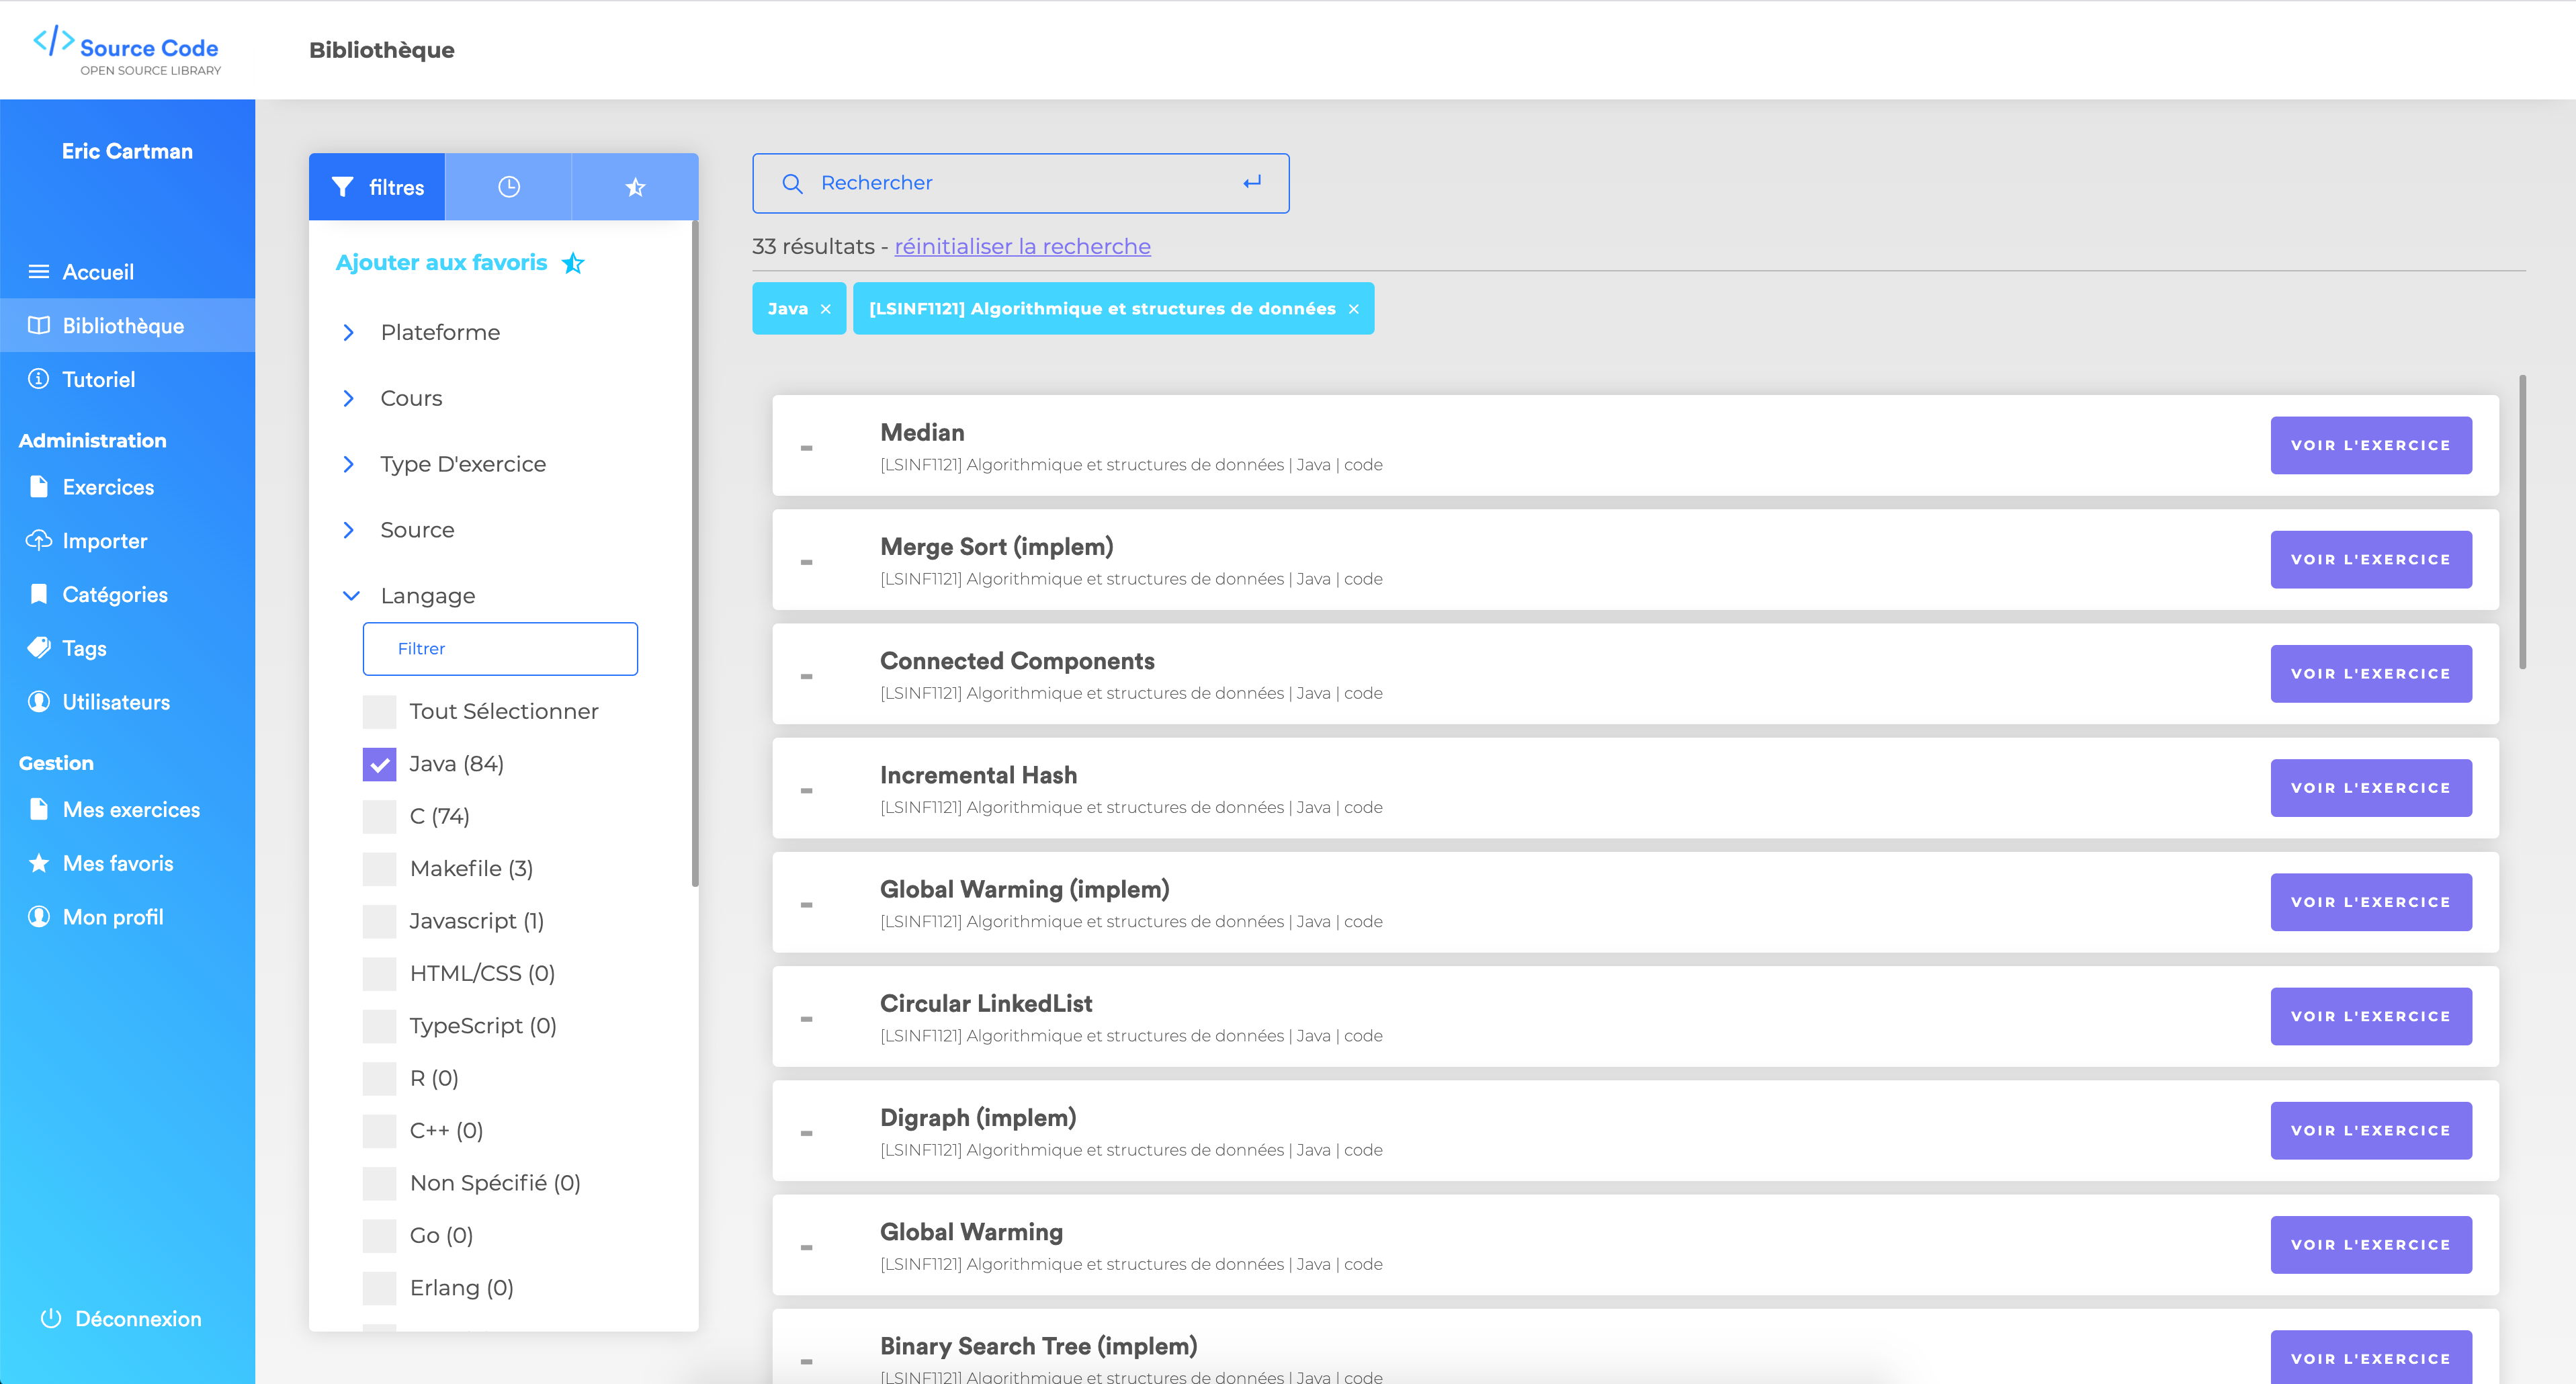
\includegraphics[width=\textwidth,height=\textheight,keepaspectratio]{images/client/search-library.png}
    \centering
    \caption[SourceCode : page bibliothèque]{page bibliothèque}
\end{figure}

\subsubsubsection{Preview d'une \gls{resinfo}}

La section de droite représente tous les exercices correspondants aux critères de recherche. Il suffit de scroller dans cette section afin de charger les \glspl{resinfo} suivantes.\\

Le preview d'une ressource contient les informations suivantes :

\begin{itemize}
    \item Le titre de la ressource
    \item Quelques \glspl{tag} que nous jugeons récurrents et pertinents pour mieux identifier le type de ressource (si référencés sur celle-ci) : 
    \begin{itemize}
        \item Le cours
        \item Le langage
        \item La difficulté
        \item La thématique
        \item Le type d'exercice
    \end{itemize}
    Nous avons choisi 5 \glspl{tag} maximum à afficher pour que le preview de la ressource soit toujours facilement visible. Pour la justification du choix des \glspl{tag}, nous l'expliquons en annexe \ref{annexe:AnalyseBiblio}, table 4.3 avec quelques éléments récurrents que nous avons pu identifier avec les autres normes.
    Les autres \glspl{tag} seront consultables depuis l'interface de la \gls{fiche} (cf. section \ref{section:ficheResInfo})
    \item La cotation de la ressource (sur 5). Nous détaillons d'ailleurs son utilité dans la section suivante (\ref{section:ficheResInfo}).
\end{itemize}

\subsubsubsection{Le panneau à onglets}
\label{section:panneau}

Pour effectuer une recherche dans la bibliothèque, il suffit de taper un titre dans la barre de recherche et/ou d'utiliser le panneau à onglets (élément central de la recherche).\\

Il existe dès lors 3 types d'onglets :

\paragraph{Filtres} Ils permettent d'affiner la recherche de \glspl{resinfo}. Les \glspl{tag} cochés apparaitront juste au-dessus des résultats. Si un \gls{tag} ne convient plus à la recherche, il suffit de décocher un des tags en question ou de cliquer sur la croix du label représentant le \gls{tag} sélectionné.\\

Comme vous pourrez le constater sur la figure \ref{figure:rechercheBibliotheque}, le panneau de filtres n'est plus à la même position que ce que nous avions imaginé avec notre patchwork \ref{figure:patchwork}. Dans ce dernier, nous avions intégré le filtrage de \glspl{tag} dans une interface dédiée à cet effet.\\

Dans l'interface actuelle, nous voulions que tout soit facilement accessible compte tenu du fait que nous allions intégrer l'historique et le système de favori au même endroit (ce que nous n'avions pas encore décidé au stade du patchwork).\\

La page que nous avions prévue sur le patchwork pour les filtres (figure \ref{figure:systemeDeFiltres}) s'apparente plutôt à une interface avancée. Nous expliquerons d'ailleurs les quelques pistes d'améliorations qui pourraient être apportées à ce sujet dans une prochaine mise à jour de la plateforme en chapitre \ref{chapter:pourAllerPlusLoin}.

Le système de filtres fonctionne comme \textit{Hackerrank} et \textit{Coderbyte} (section \ref{section:situation}) :

\begin{itemize}
    \item Plusieurs \glspl{tag} peuvent être choisis dans une même catégorie. Dans ce cas, la recherche donnera des résultats comprenant au moins un des \glspl{tag} sélectionnés.
    \item Lorsqu'un \gls{tag} est sélectionné dans deux catégories différentes, la recherche prendra en compte toutes les \glspl{resinfo} comprenant au moins un \gls{tag} sélectionné dans chacune des catégories.
\end{itemize}

Si vous possédez un compte, vous pouvez enregistrer les critères de recherche actuels en cliquant sur "Ajouter aux favoris". Après avoir fourni un nom pour le favori, ce dernier apparaitra désormais dans l'onglet favoris.\\

\paragraph{Historique} L'historique vous permet de naviguer à travers les recherches que vous avez précédemment effectuées. Il restera disponible tout au long de la session, après quoi il sera réinitialisé.\\

L'historique affiche les recherches précédemment effectuées, de la plus récente à la plus ancienne. Le titre de recherche s'affichera en bleu tandis que les \glspl{tag} sélectionnés seront affichés en mode "pêle-mêle", séparés par une barre verticale (|).\\

\paragraph{Favoris (seulement lorsqu'on est connecté)} Les favoris créés apparaitront dans ce panneau. Pour utiliser un des favoris, il suffit de cliquer sur l'un d'eux et la recherche s'actualisera depuis la même page avec les nouveaux critères de recherche pris en compte.

Vous pouvez supprimer ou modifier les favoris depuis ce panneau en passant la souris sur un favori, puis en sélectionnant une des deux icônes qui s'affichent.

\begin{itemize}
    \item \textbf{Le crayon} permet de modifier le favori. Il mènera donc sur la page de modification de ce favori (voir section \ref{section:gestionFavorite}).
    \item \textbf{La poubelle} permet de supprimer le favori directement depuis le panneau.
\end{itemize}

\subsubsection{La \gls{fiche} d’une \gls{resinfo}}
\label{section:ficheResInfo}

Les \glspl{resinfo} sont le cœur de \texttt{SourceCode}. Elles représentent toutes les contributions émises par la communauté. Elles peuvent être consultées depuis la bibliothèque en cliquant sur "voir l'exercice".\\

Voici à quoi ressemble la structure d'une \gls{fiche} :

\begin{figure}[H]
    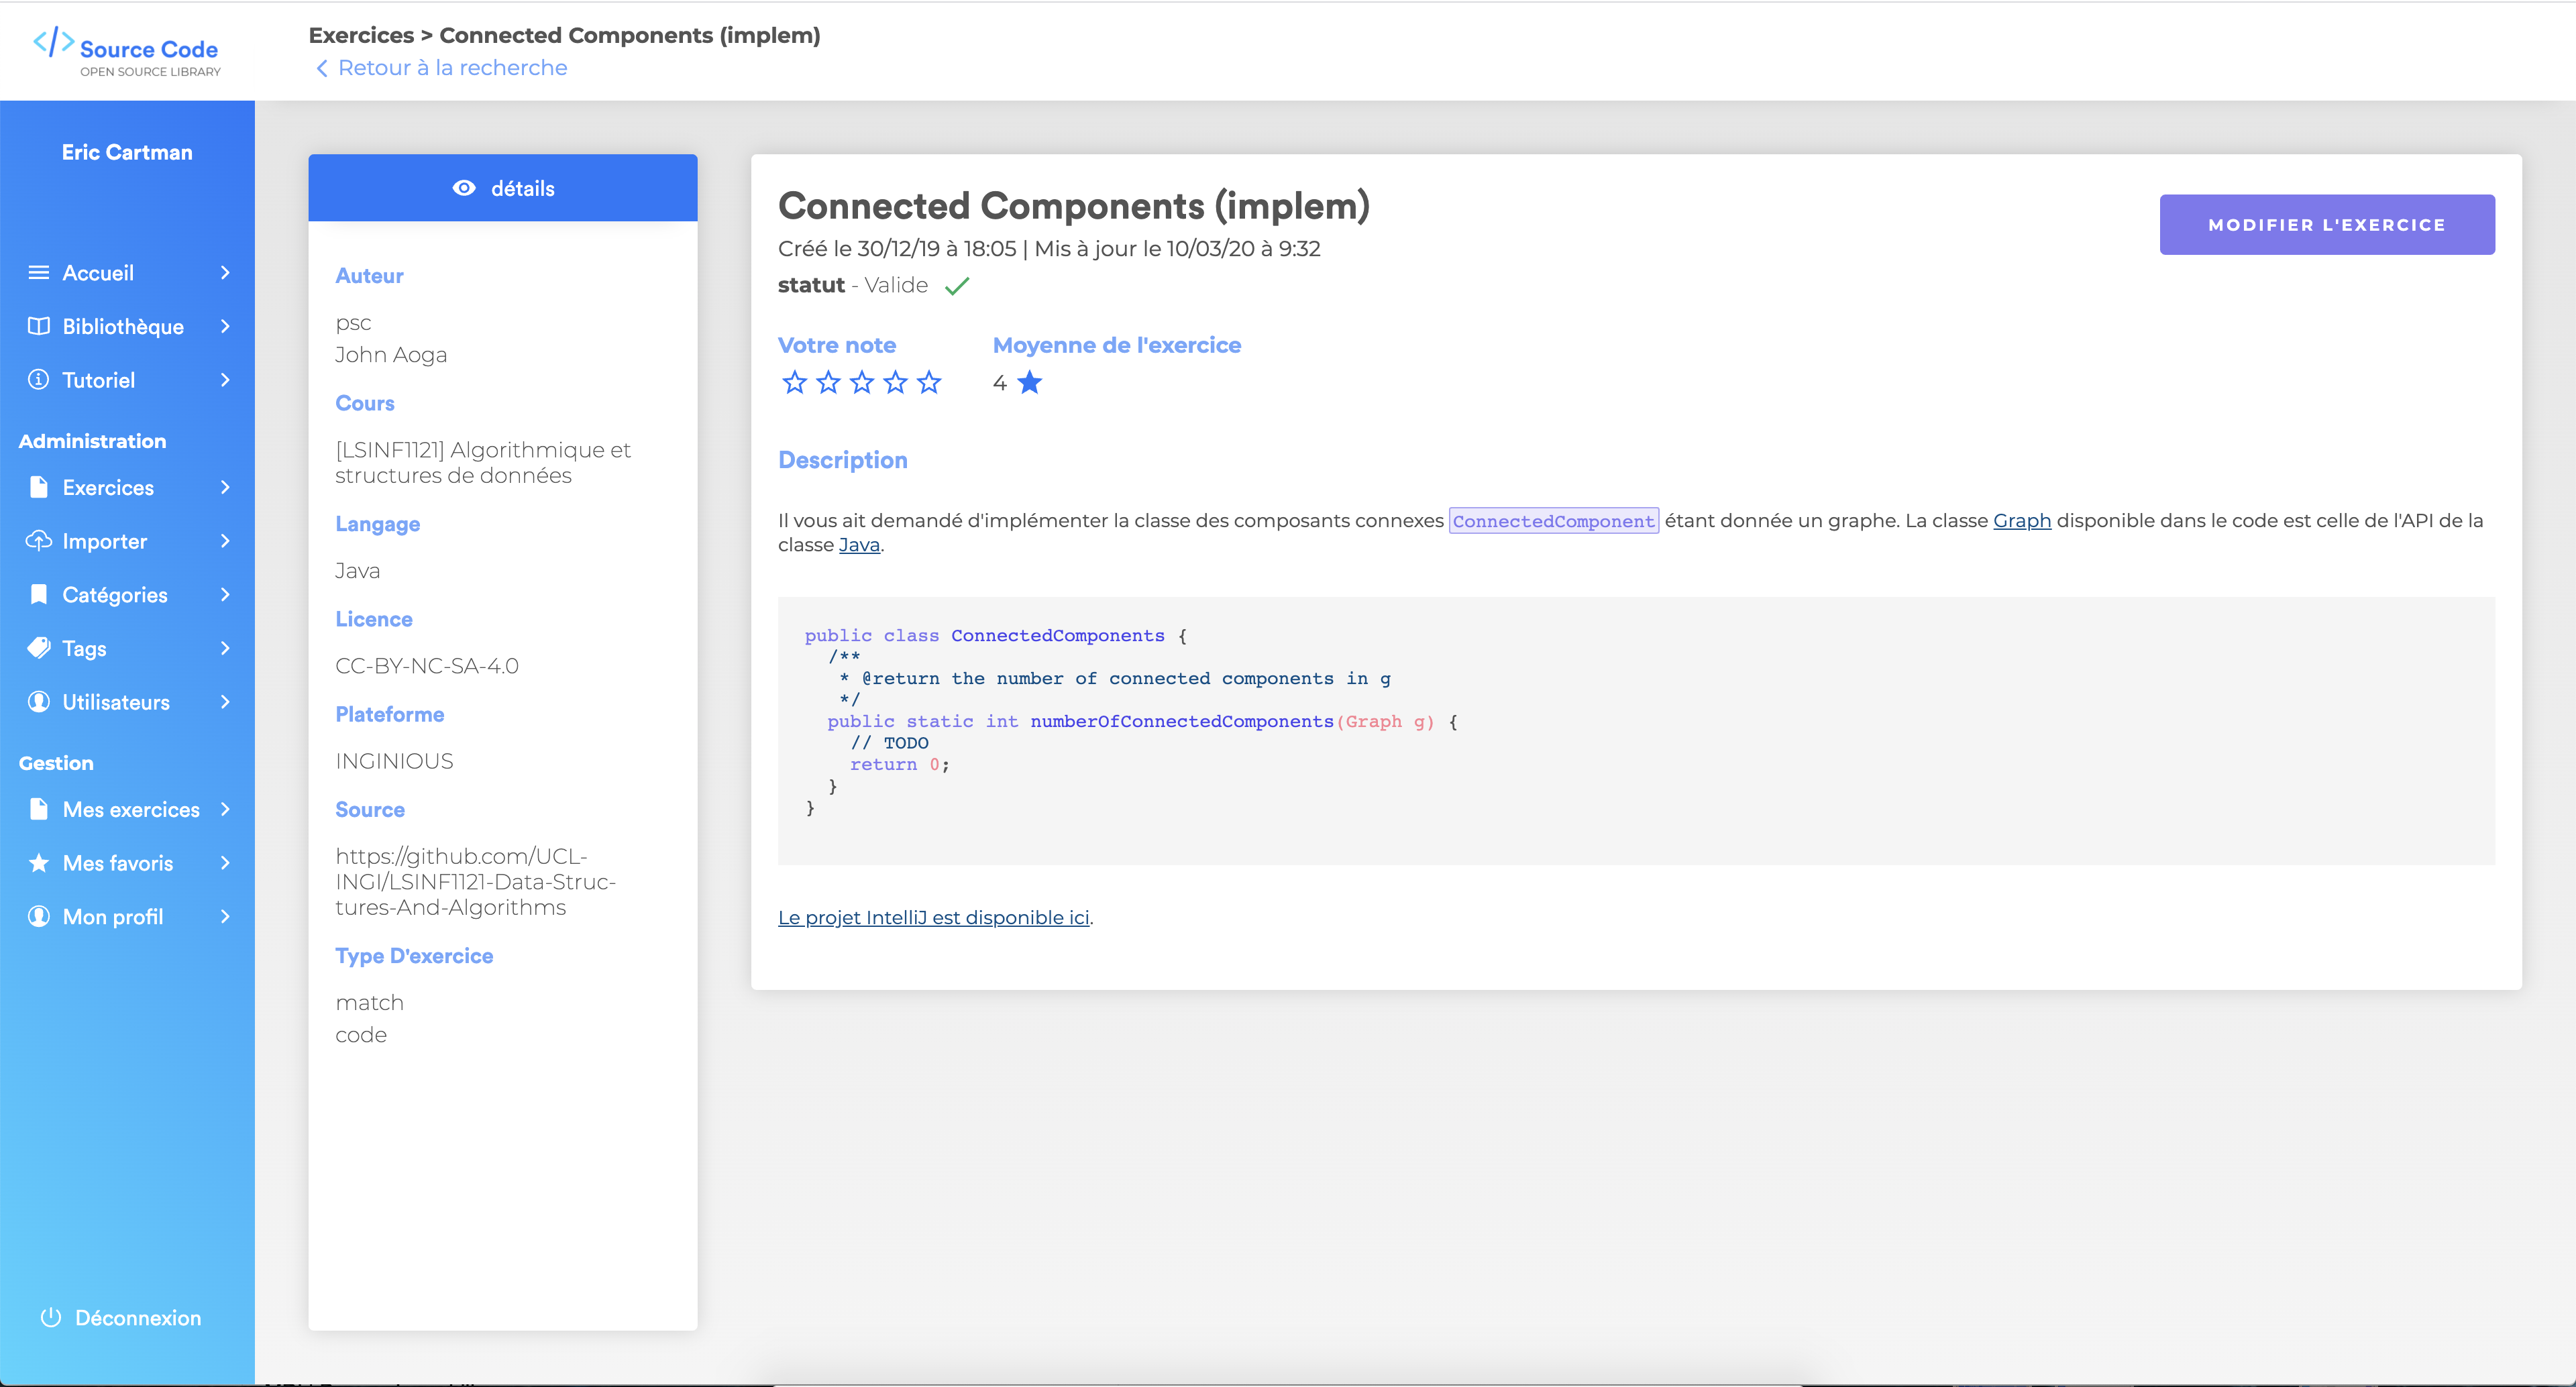
\includegraphics[width=\textwidth,height=\textheight,keepaspectratio]{images/client/fiche.png}
    \centering
    \caption[SourceCode : la représentation d'une \gls{fiche}]{la représentation d'une \gls{fiche}}
\end{figure}

Lorsque la ressource vous appartient ou que vous êtes un administrateur, un bouton de modification apparait dans le coin supérieur droit de la \gls{fiche} de la ressource. Cliquer sur le bouton mènera sur le formulaire de modification de la ressource (voir section \ref{section:gestionResInfo} pour la gestion côté utilisateur ou voir section \ref{section:resInfoAdmin} pour la gestion côté (super-)administrateur).\\

\subsubsubsection{Panneau de détails}

Le panneau latéral contient tous les \glspl{tag} qui ont été ajoutés pour identifier la ressource. Plus il y en a, plus cette dernière sera favorablement référencée sur la plateforme.\\

En effet, la recherche dans la bibliothèque fonctionne avec les filtres (\glspl{tag}) et/ou le titre de recherche. Plus le titre de la ressource sera pertinent, plus facile elle pourra être retrouvée en tapant une partie du titre dans la barre de recherche. 
De la même manière, plus la \gls{resinfo} contient de \glspl{tag} dans des \glspl{tagCat} différentes, plus il sera facile de la retrouver avec le panneau de filtres. Il est donc important que le créateur de la \gls{fiche} fasse preuve d'exhaustivité dans le choix des \glspl{tag} et de pertinence. Le cas échéant, les administrateurs se réservent le droit d'invalider la ressource ou de la laisser passer, sans grande chance d'être retrouvée par d'autres utilisateurs de la plateforme.

\subsubsubsection{Système de vote}

Sur la \gls{fiche} de la \gls{resinfo}, vous pouvez donner une note sur la qualité de la ressource sur 5 étoiles. Il suffit de cliquer sur une des étoiles pour donner un score (seulement si vous possédez un compte).\\

Là aussi, le vote joue un rôle important dans le référencement de la \gls{resinfo} car les utilisateurs peuvent filtrer les \glspl{resinfo} en fonction de leur note.\\

Nous avons choisi un système de vote sur 5 étoiles, car notre analyse (section \ref{section:situation}) a révélé cette caractéristique commune sur de nombreux sites. La plateforme \textit{Hackerrank} utilise d'ailleurs ce système.


\subsection{Gestion}

Le module de gestion comprend :

\begin{itemize}
    \item La gestion de \glspl{resinfo} personnelles (\textit{mes-exercices/})
    \item La gestion de favoris (\textit{mes-favoris/})
    \item La consultation du profil (\textit{profil})
\end{itemize}

Ce module est accessible aux utilisateurs (possédant un compte) et aux administrateurs.

\begin{figure}[H]
    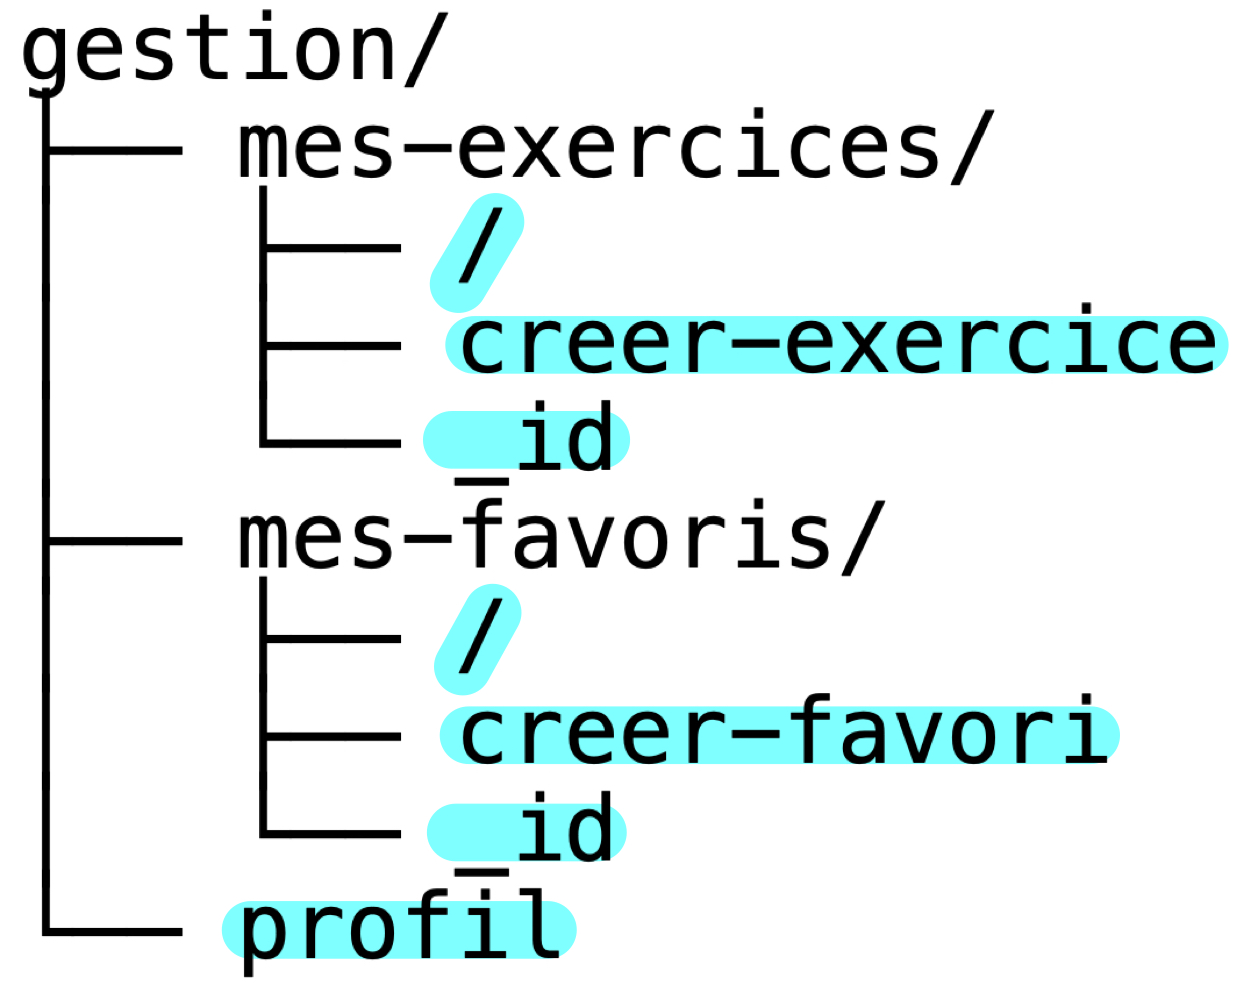
\includegraphics[width=\textwidth,height=0.2\textheight,keepaspectratio]{images/client/gestion.jpeg}
    \centering
    \caption[SourceCode : module de gestion (URL)]{Module de gestion (URL)}
\end{figure}

\subsubsection{Gestion de \glspl{resinfo} personnelles}
\label{section:gestionResInfo}

La recherche fonctionne de la même manière que dans la bibliothèque, à la différence qu'elle est effectuée dans les \glspl{resinfo} personnelles seulement. Pour comprendre le fonctionnement du panneau à onglets, consultez la section \ref{section:panneau}.

\begin{figure}[H]
    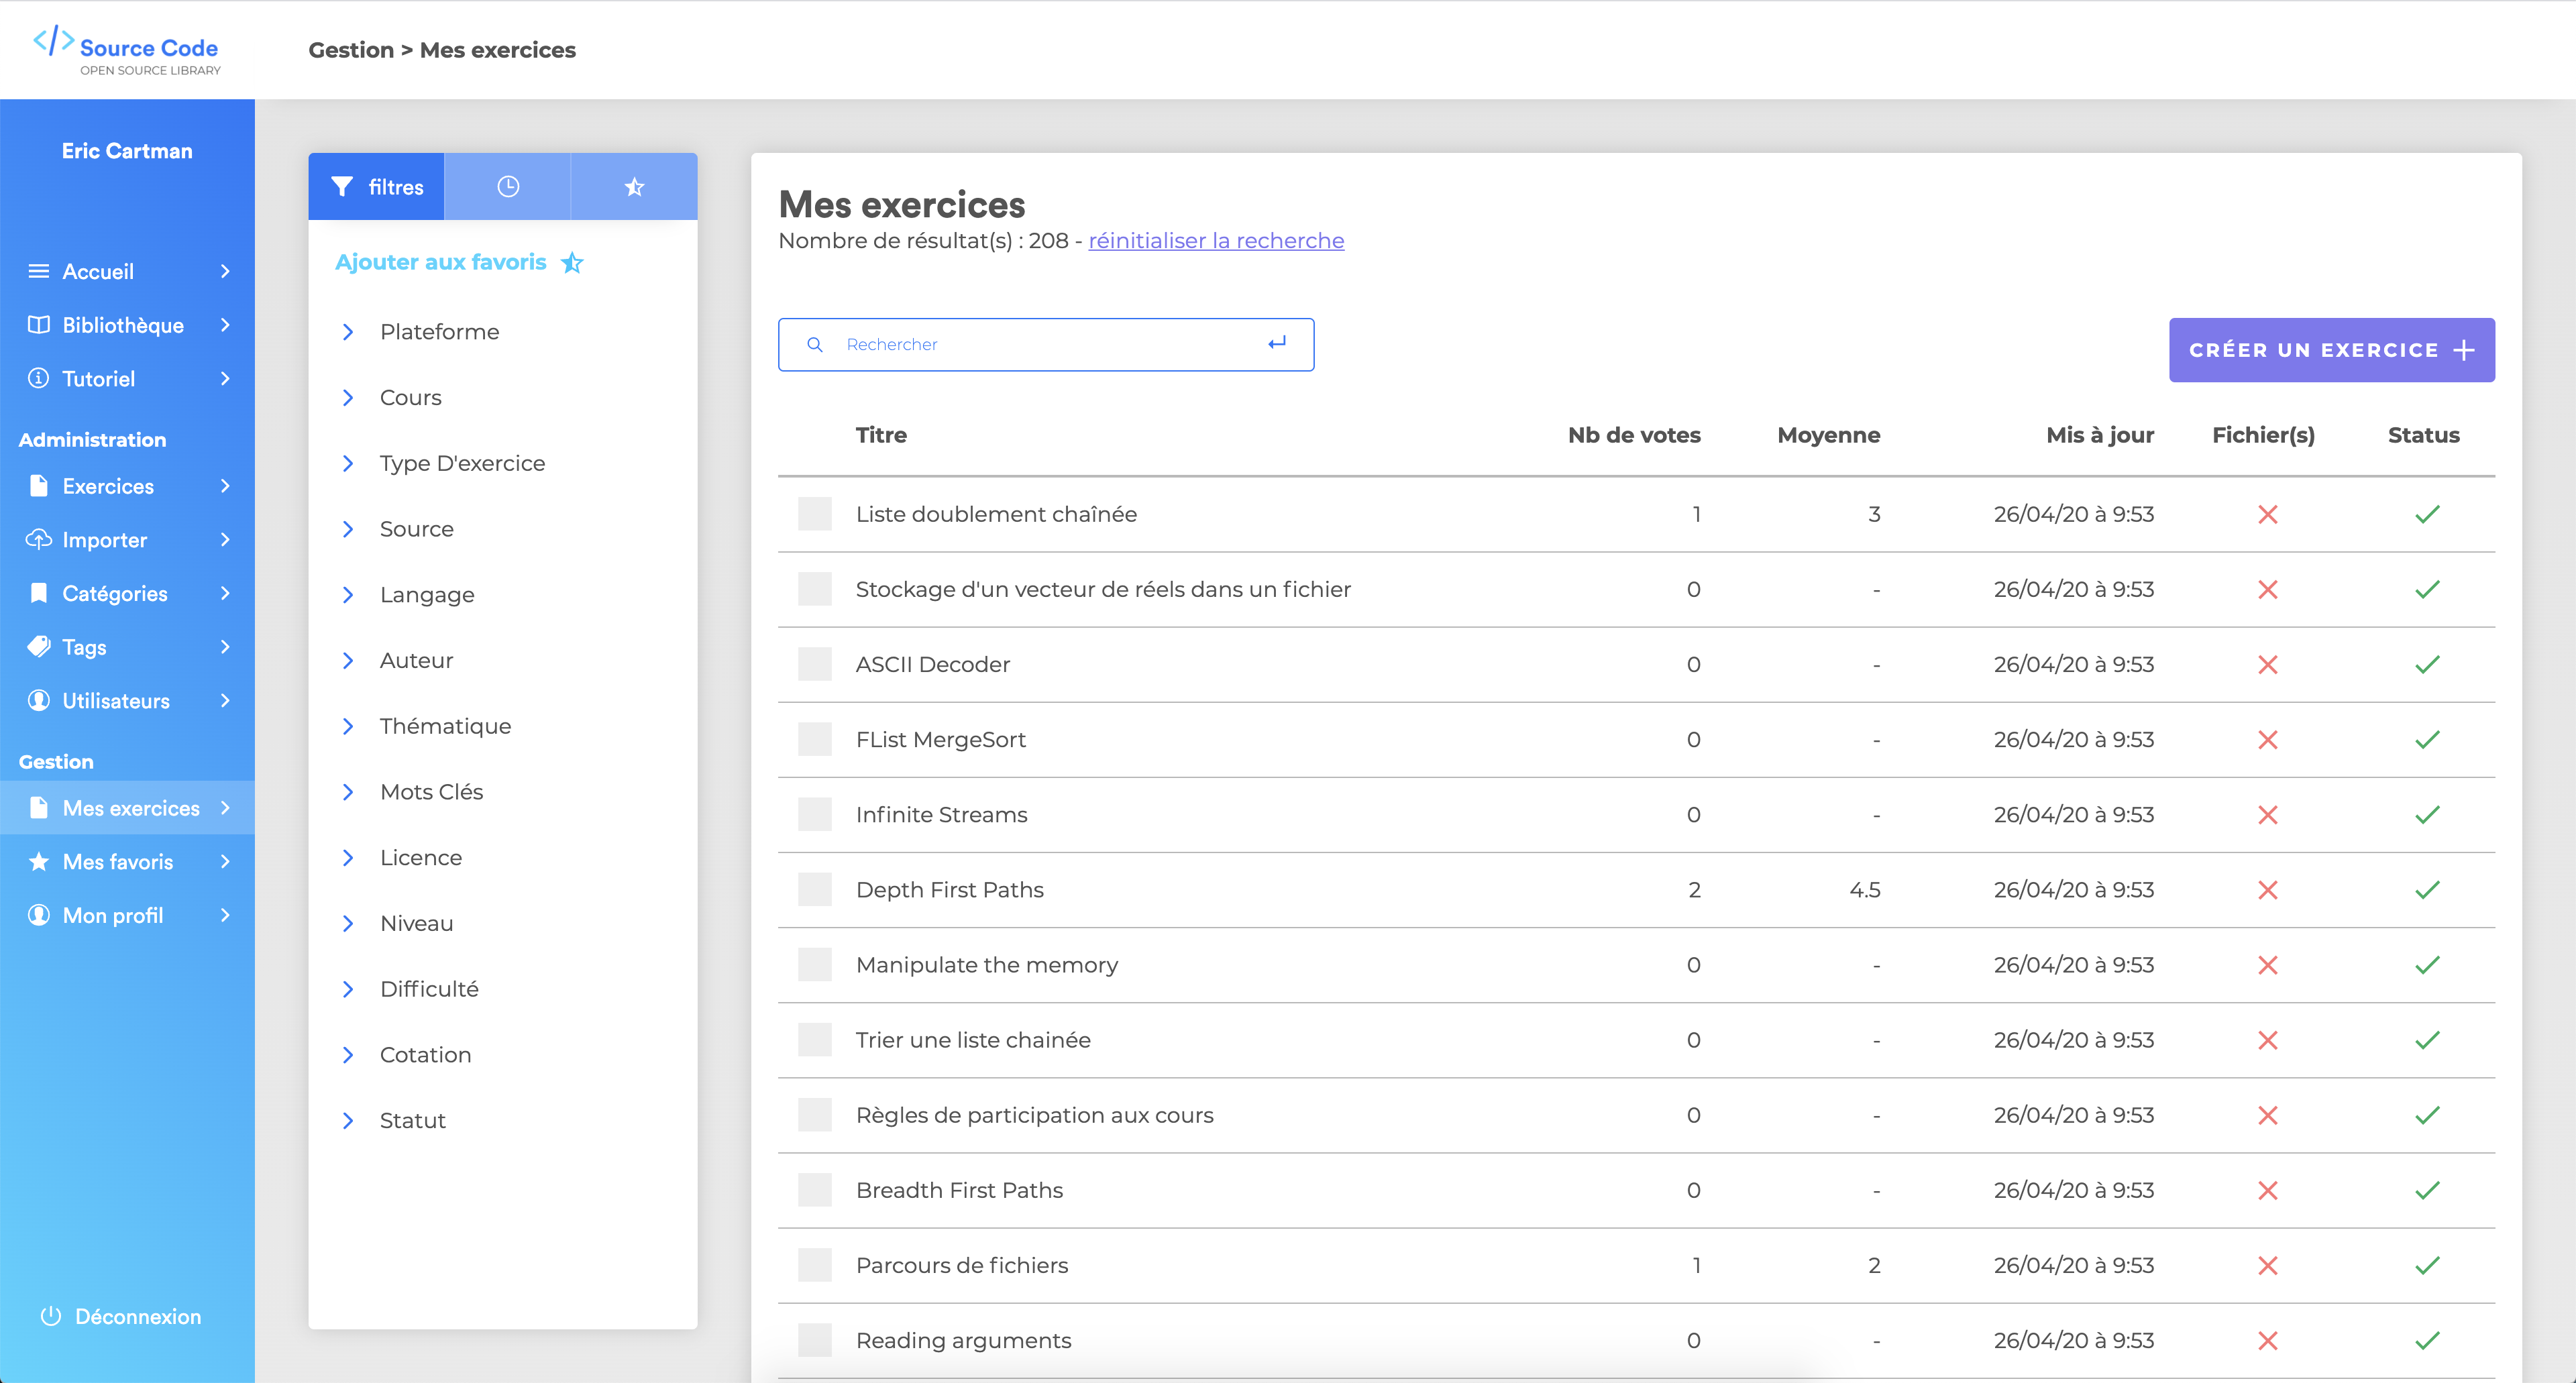
\includegraphics[width=\textwidth,height=\textheight,keepaspectratio]{images/client/gestion-exercices.png}
    \centering
    \caption[SourceCode : gestion des \glspl{resinfo} personnelles]{Gestion des \glspl{resinfo} personnelles (mes-exercices/)}
\end{figure}

Plusieurs informations sont disponibles pour identifier les ressources informatiques :

\begin{itemize}
    \item Le titre de la ressource
    \item Le nombre de votes émis par la communauté
    \item La moyenne (sur 5) des votes émis par la communauté
    \item La date de mise à jour de la ressource informatique
    \item La présence d'une archive zip pour la ressource informatique
    \item Le statut de la ressource
\end{itemize}


\subsubsubsection{Statuts d'une \gls{resinfo}}
\label{section:statutDuneRessource}

Nous prêtons attention à la qualité du contenu sur la plateforme. Nous avons donc mis en place un système de statuts pour donner une indication sur l'état d'une \gls{resinfo}.\\

Voici les différents états que peut prendre la \gls{resinfo} (découle de notre analyse bibliographique en annexe \ref{annexe:AnalyseBiblio}) :

\begin{itemize}
    \item 
\includegraphics[valign=b,height=1.4\fontcharht\font`X]{images/client/draft.png} \textbf{Brouillon}
    \begin{itemize}
        \item Signifie que la ressource n'est pas encore prête à être validée par l'administration. La ressource n'est donc pas disponible depuis la bibliothèque et uniquement accessible depuis l'interface de gestion du créateur de la \gls{fiche} et des administrateurs.
    \end{itemize}
    \item 
\includegraphics[valign=b,height=1.4\fontcharht\font`X]{images/client/pending.png} \textbf{En attente de validation}
    \begin{itemize}
        \item La ressource est mise en attente pour révision. Un administrateur se chargera de la valider ultérieurement.
    \end{itemize}
    \item 
\includegraphics[valign=b,height=1.4\fontcharht\font`X]{images/client/validated.png} \textbf{Valide}
    \begin{itemize}
        \item Lorsque la ressource est acceptée par l'administration, la ressource est alors validée et disponible publiquement depuis la bibliothèque.
    \end{itemize} 
    \item 
\includegraphics[valign=b,height=1.4\fontcharht\font`X]{images/client/not-validated.png} \textbf{Invalide}
    \begin{itemize}
        \item Lorsque la ressource n'est pas considérée comme valide (mauvaise qualité d'écriture, doublons, incohérences), l'administrateur se réserve le droit d'invalider la ressource. Elle pourra néanmoins être modifiée pour la refaire passer en phase de révision.
    \end{itemize}
    \item 
\includegraphics[valign=b,height=1.4\fontcharht\font`X]{images/client/archive.png} \textbf{Archive}
    \begin{itemize}
        \item Quand une ressource est archivée, elle est alors uniquement accessible par les administrateurs et par son créateur.
    \end{itemize}
\end{itemize}

Le diagramme UML pour l'état d'une \gls{resinfo} se retrouve en figure \ref{pic:stateDiagramForFiches}.

\subsubsubsection{Gestion du statut de la ressource}

Pour modifier l'état d'une ou plusieurs ressources, il faut dans un premier temps les cocher. Une liste déroulante d'actions apparaitra à côté du bouton de création d'exercices avec les options suivantes :

\begin{itemize}
    \item Publier (envoyer pour révision)
    \item Mettre en brouillon
    \item Archiver
\end{itemize}

Plus d'options seront disponibles pour les administrateurs, car il est évident qu'un utilisateur ne puisse pas valider sa propre ressource par exemple.

\begin{figure}[H]
    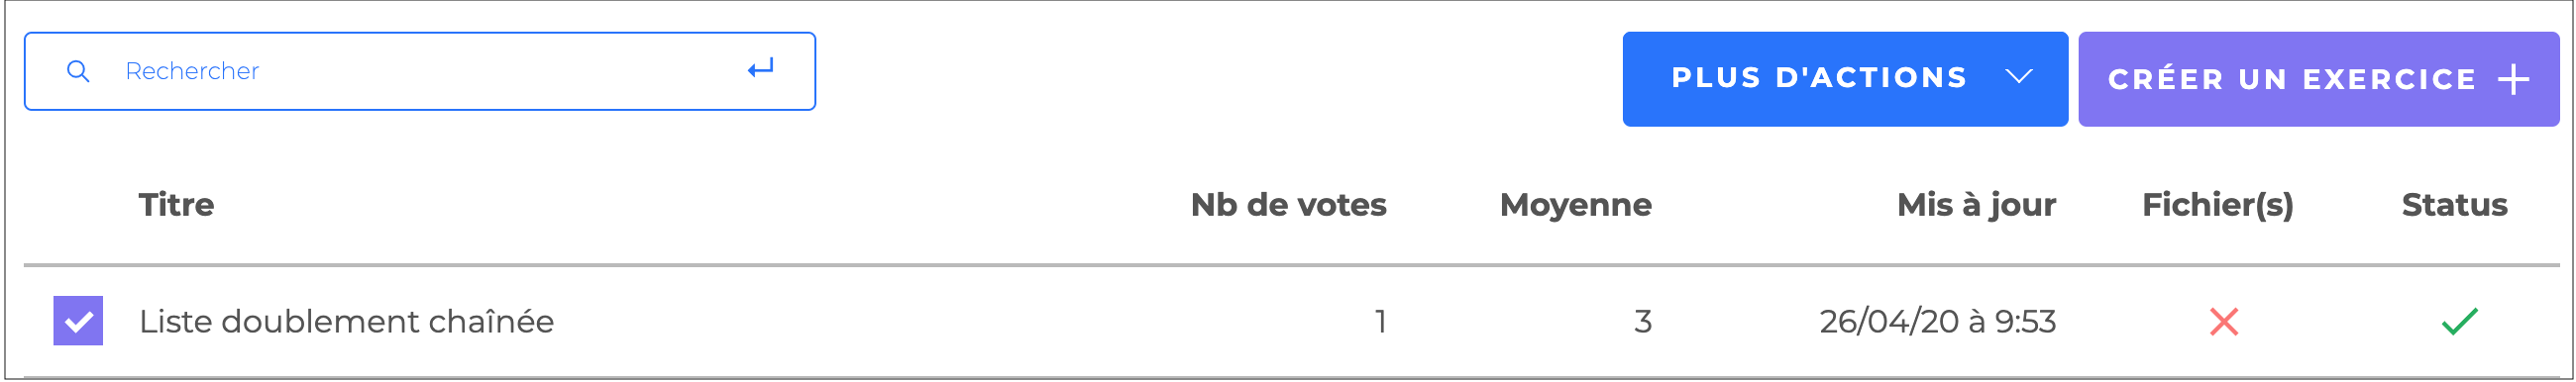
\includegraphics[width=\textwidth,height=\textheight,keepaspectratio]{images/client/gestion-options.png}
    \caption[SourceCode : créer une \gls{resinfo}]{Gestion des \glspl{resinfo} personnelles (creer-exercice ou \_id)}
    \centering
\end{figure}

\subsubsection{Création/modification d'une ressource}

La fiche d'une \gls{resinfo} est composée des éléments suivants :

\begin{itemize}
    \item Un titre (obligatoire)
    \item Une description (obligatoire)
    \item Des \glspl{tag} (obligatoire)
    \item Une archive zip en guise de fichier
    \item Un lien externe (URL)
\end{itemize}

\begin{figure}[H]
    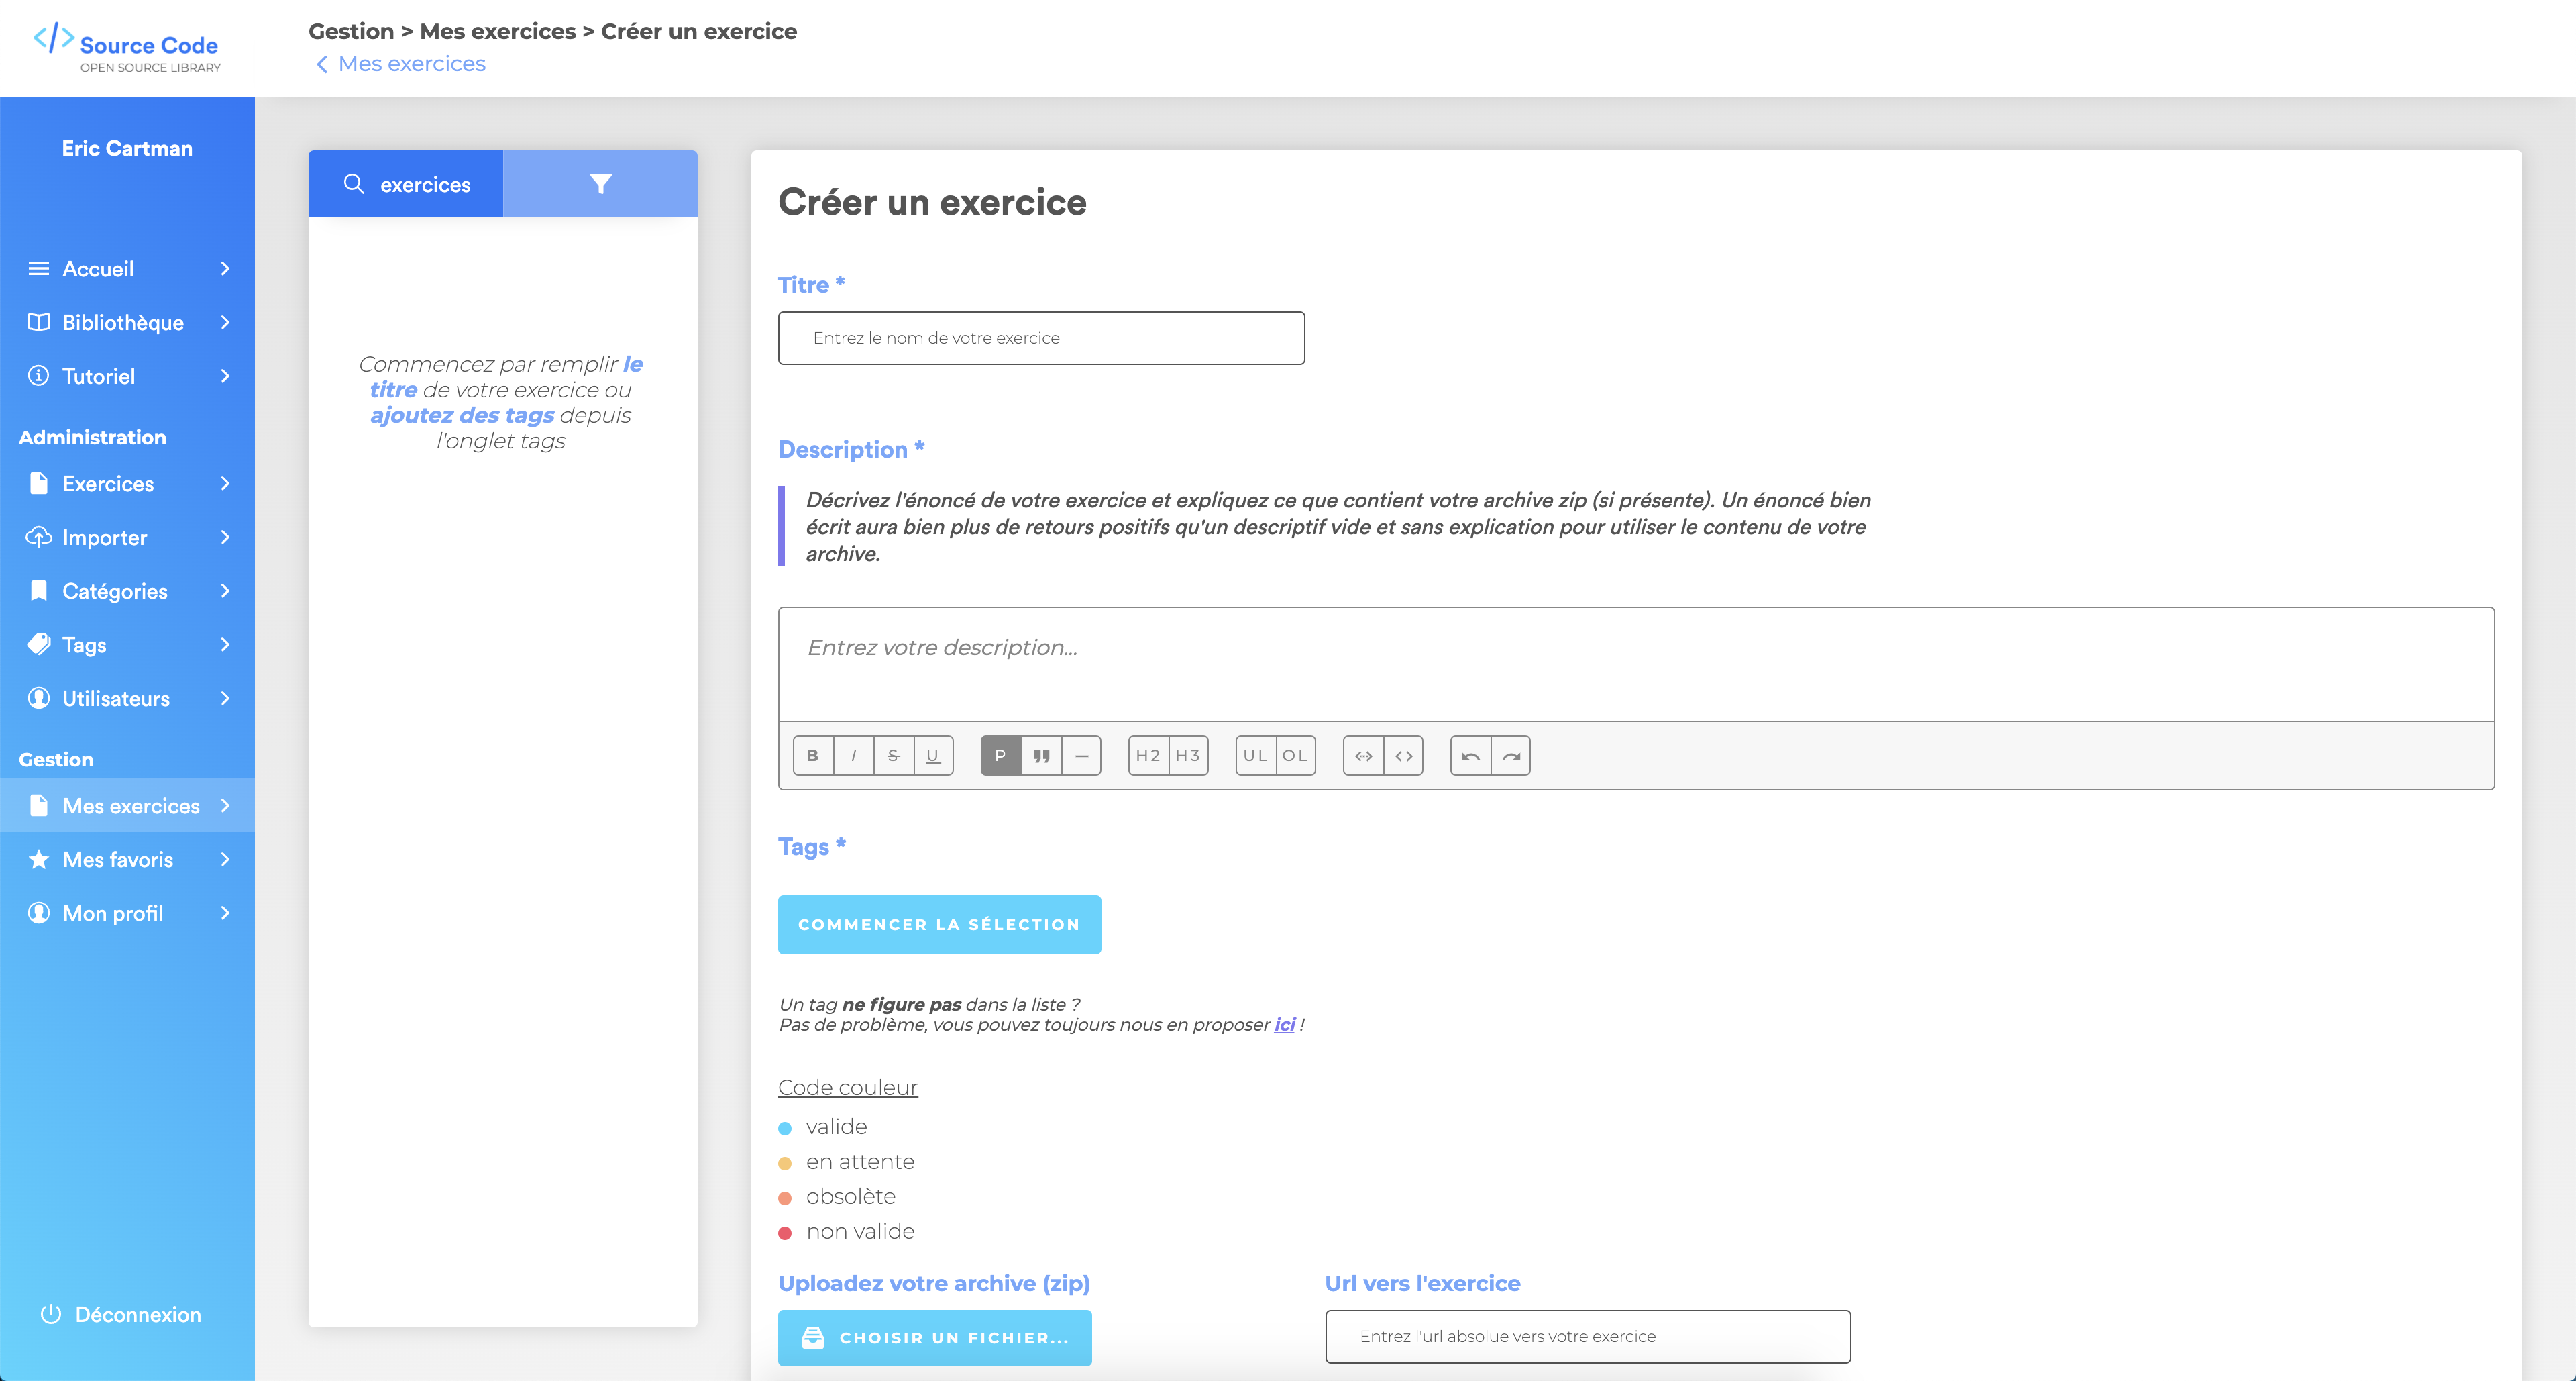
\includegraphics[width=\textwidth,height=\textheight,keepaspectratio]{images/client/create-exercise.png}
    \centering
\end{figure}

Lorsque vous remplissez le champ titre et/ou ajoutez des tags, le panneau à onglets "exercices" affiche toutes les \glspl{resinfo} similaires (au sens strict) à la \gls{fiche} que vous créez. Cela signifie que toutes les \glspl{resinfo} contenant le titre entré et TOUS les \glspl{tag} que vous avez référencés seront ainsi présents dans ce panneau.

\begin{figure}[H]
    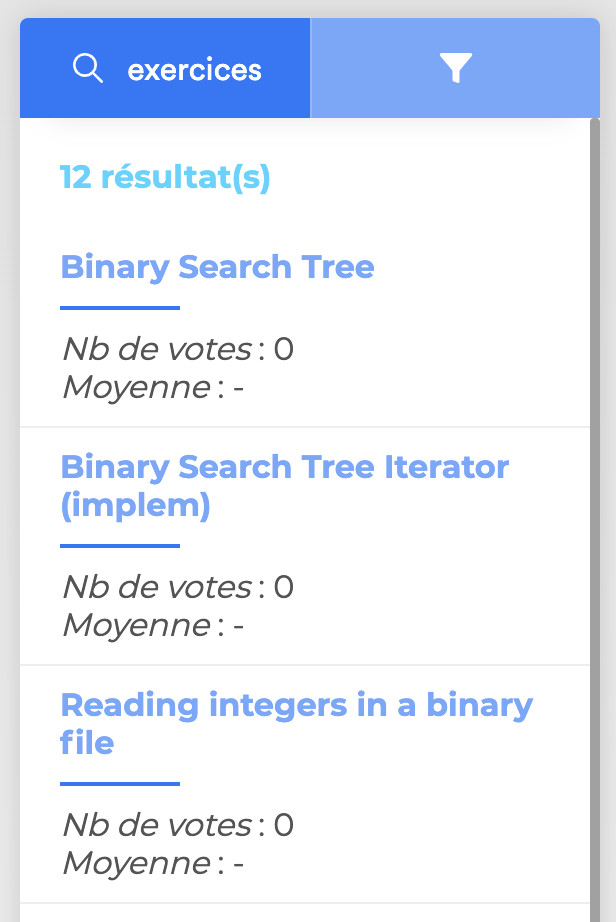
\includegraphics[width=\textwidth,height=0.3\textheight,keepaspectratio]{images/client/similarity.png}
    \centering
\end{figure}

\subsubsubsection{Soumission de la ressource}

Deux options de soumission sont disponibles :

\begin{itemize}
    \item \textbf{Brouillon :} Vous estimez que la \gls{resinfo} n'est pas encore prête pour être validée, vous la laissez donc en stand-by pour la modifier plus tard. À noter que vous \textbf{DEVEZ} remplir les champs obligatoires pour l'enregistrer sous cet état. Il s'agit d'un choix technique décidé au niveau de l'\gls{api}, pour conserver un seuil minimal de qualité dans les contributions.
    \item \textbf{Soumettre :} Vous estimez que la \gls{resinfo} est prête pour inspection. En cliquant sur soumettre, la ressource se met automatiquement en mode "en attente", jusqu'à ce qu'un administrateur la prenne en charge pour validation. Ce texte est remplacé par \textbf{valider} dans le cas de l'administrateur. Le statut de la ressource sera ainsi valide.
\end{itemize}

Dans le cas de l'administrateur, ce dernier possède les options suivantes, en plus des précédentes :

\begin{itemize}
    \item \textbf{Invalider :} Vous estimez que la \gls{resinfo} n'est pas correcte, car elle comporte des défauts, des incohérences ou est un dupliqué d'une autre \gls{resinfo}.
    \item \textbf{Archiver :} Vous estimez que la \gls{resinfo} n'a plus d'utilité à demeurer dans la bibliothèque. En choisissant cette option, seuls les administrateurs et le créateur de la ressource pourront consulter cette ressource dans le futur.
    \item \textbf{Mettre en attente :} Vous estimez que la \gls{resinfo} est prête pour inspection. En cliquant sur soumettre, la ressource se met automatiquement en mode "en attente", jusqu'à ce qu'un administrateur la prenne en charge pour validation.
\end{itemize}

\subsubsection{Gestion de favoris}
\label{section:gestionFavorite}

Les favoris permettent d'enregistrer des critères de recherche (titre de recherche et filtres) pour pouvoir les réutiliser par après, sans devoir parcourir le panneau de filtres pour effectuer la même recherche.\\

Pour gérer les favoris, il suffit de passer la souris sur l'un d'eux. Deux icônes apparaitront, le crayon permettant de modifier le favori et la poubelle permettant de le supprimer.

\begin{figure}[H]
    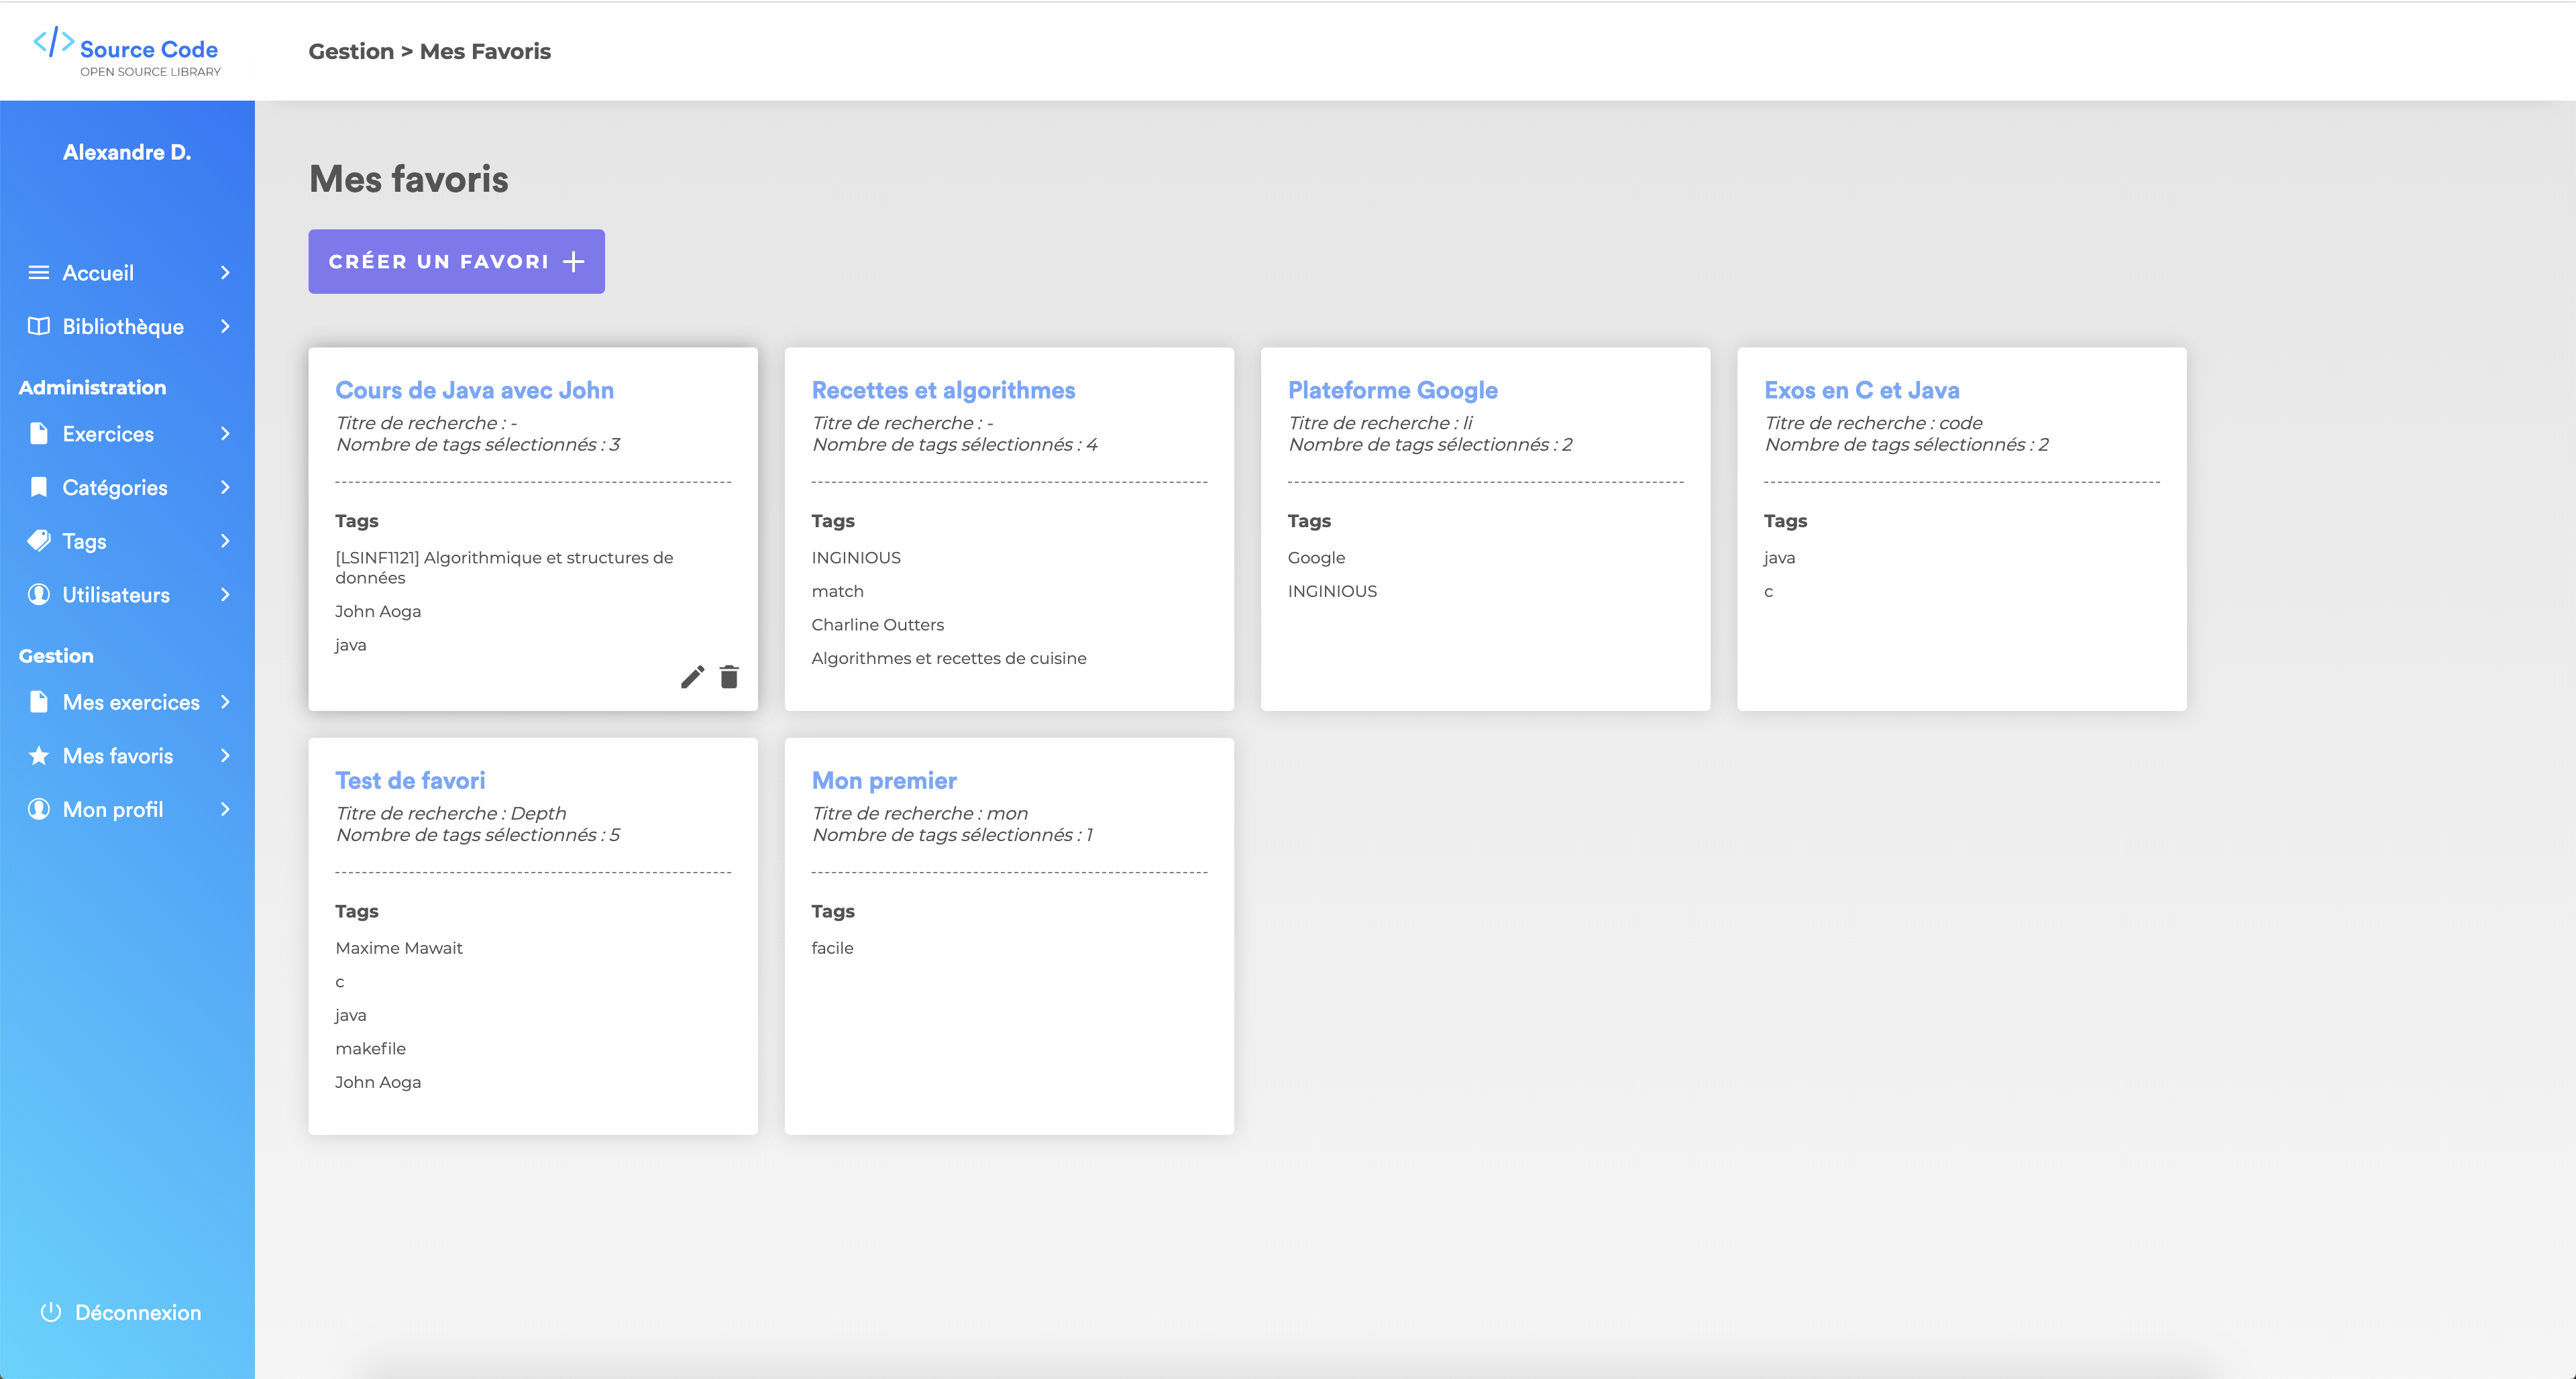
\includegraphics[width=\textwidth,height=\textheight,keepaspectratio]{images/client/gestion-favorite.png}
    \caption[SourceCode : gestion des favoris]{Gestion des favoris (mes-favoris/)}
\end{figure}

\subsubsubsection{Formulaire de création/modification d'un favori}

Voici les différents champs à remplir pour créer un favori :

\begin{itemize}
    \item \textbf{Nom du favori (obligatoire) :} donner un nom au favori.
    \item \textbf{Titre de la sélection :} titre de recherche.
    \item \textbf{\Glspl{tag} :} les tags qui vont être appliqués pour votre recherche.
\end{itemize}

\begin{figure}[H]
    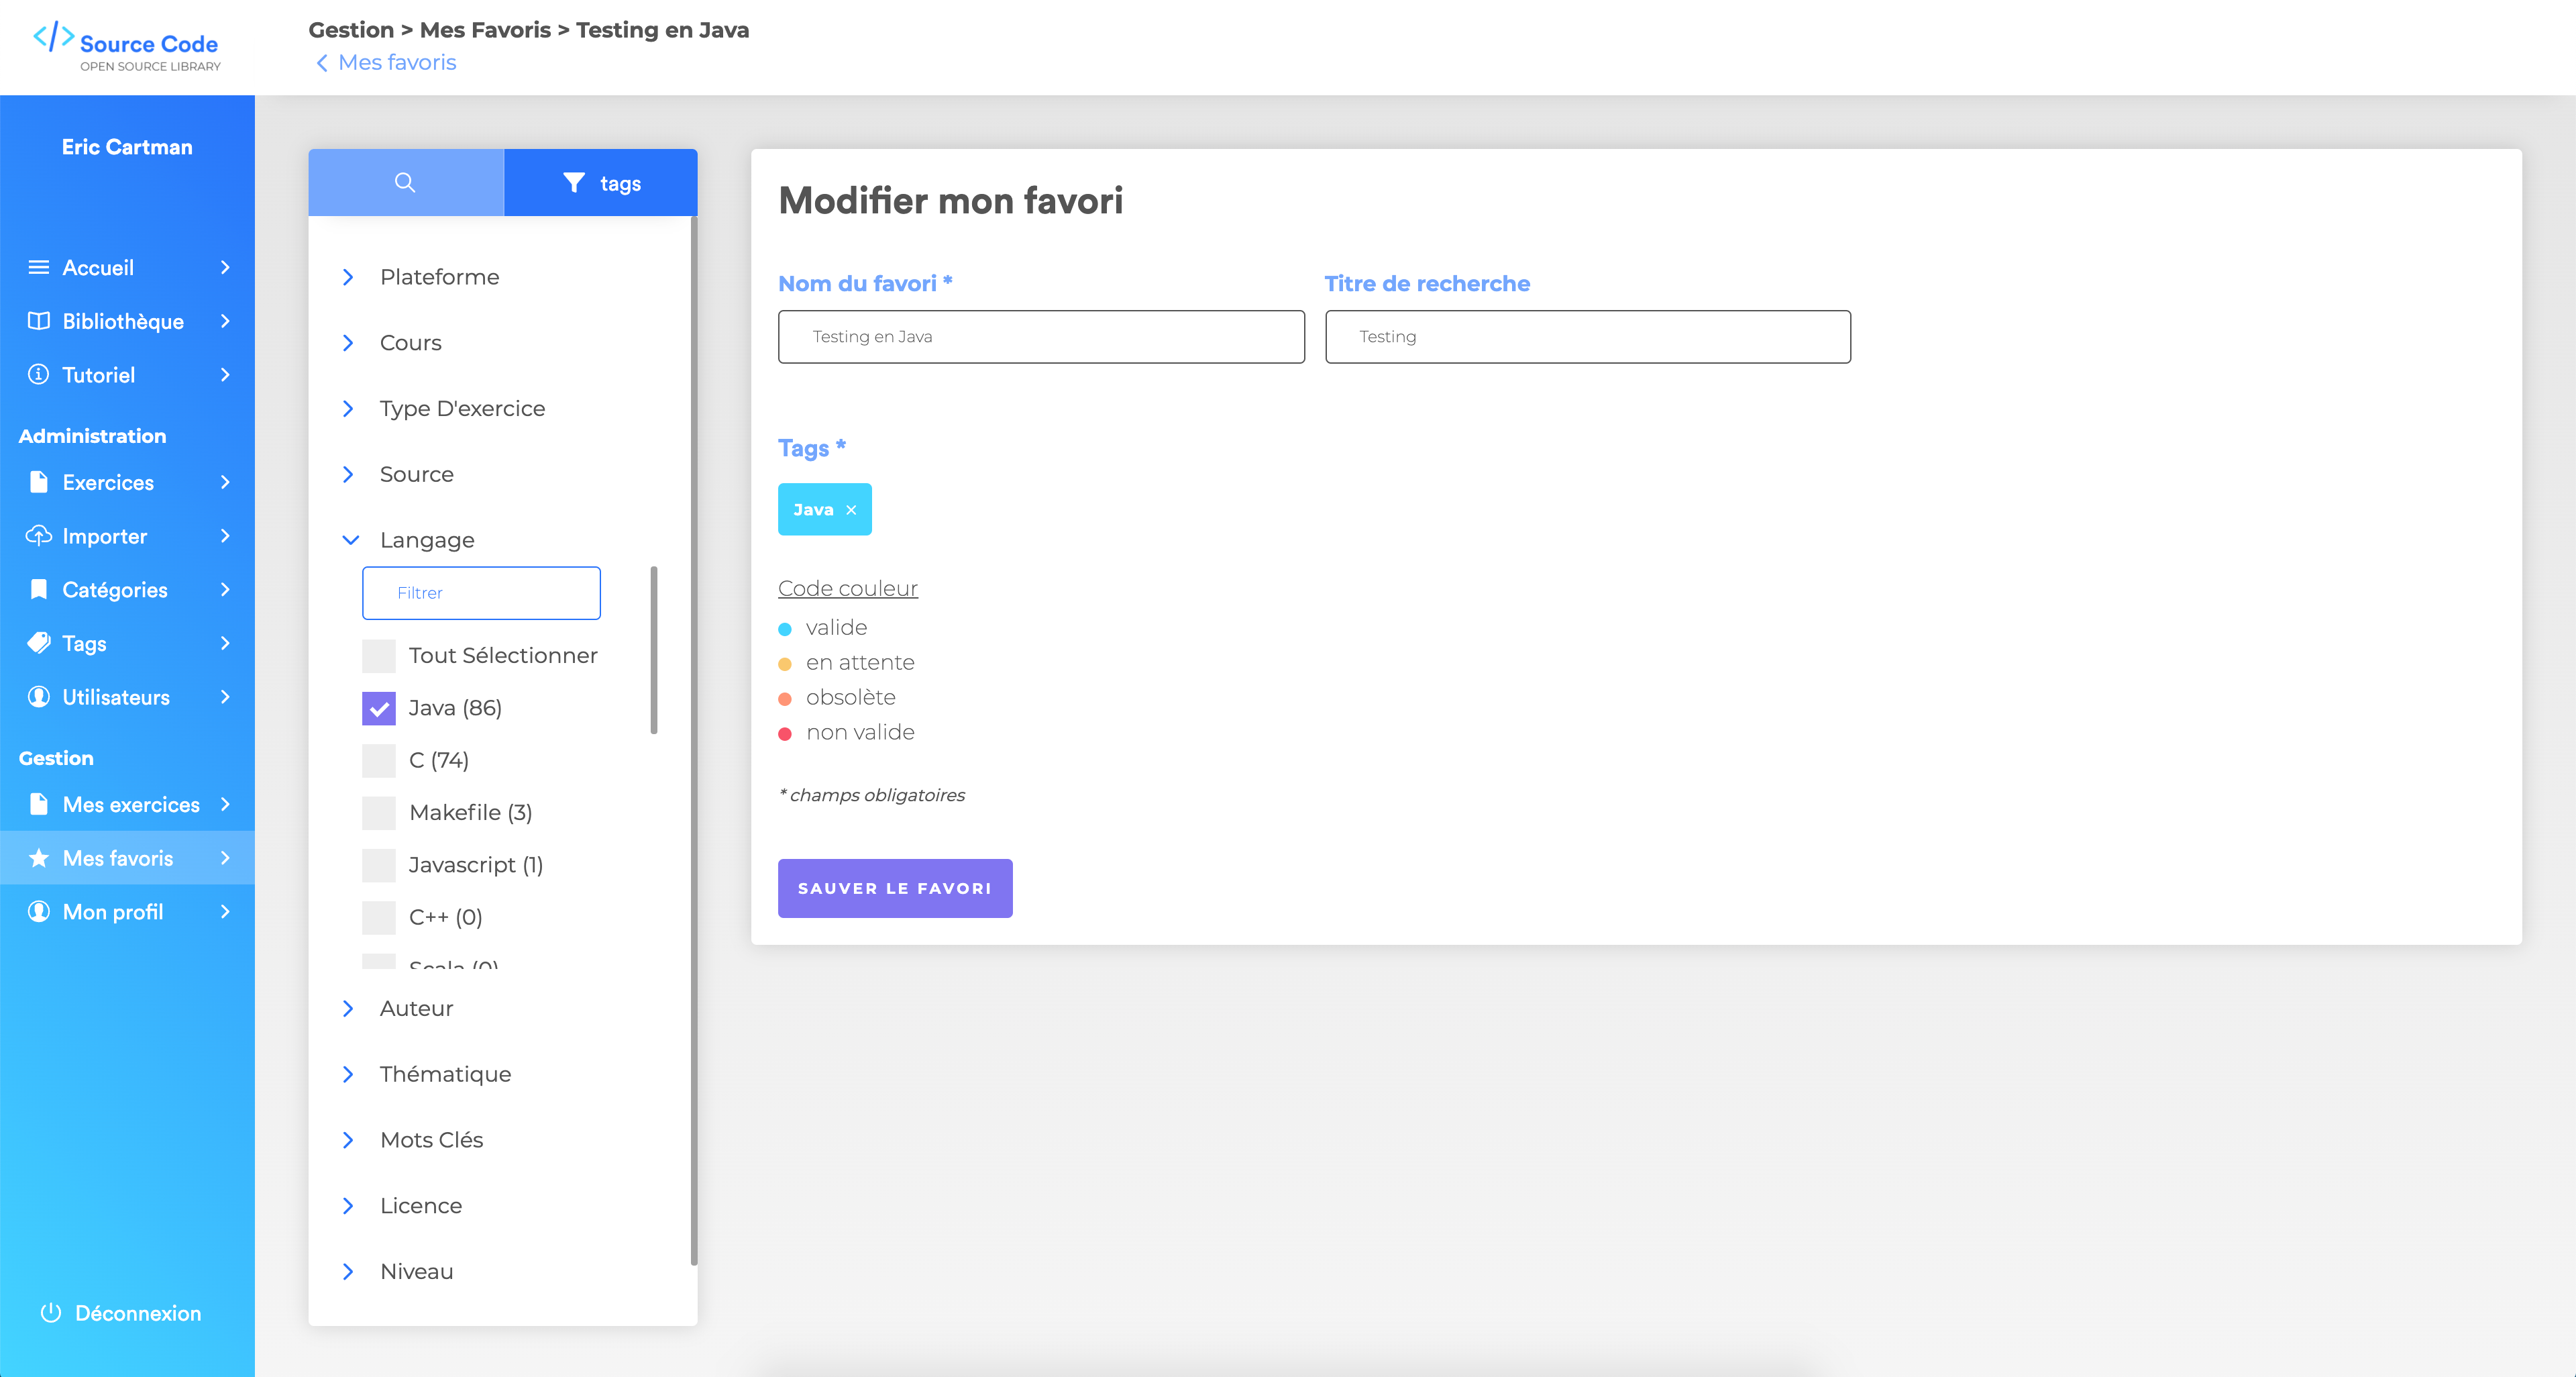
\includegraphics[width=\textwidth,height=\textheight,keepaspectratio]{images/client/favorite-form.png}
    \caption[SourceCode : création/modification des favoris]{Création/modification des favoris (creer-favori ou \_id)}
    \centering
\end{figure}

En ce qui concerne l'ajout de \glspl{tag}, un code couleur représentant leur statut est présenté (figure \ref{pic:stateDiagramForTags} pour le schéma UML à états). À noter que ce choix de statuts découle de notre analyse bibliographique en annexe \ref{annexe:AnalyseBiblio}. :

\begin{itemize}
    \item Un \gls{tag} \textbf{valide} pourra être utilisé depuis la bibliothèque pour filtrer les \glspl{resinfo}. Ceci garantit un meilleur référencement pour la ressource.
    \item Un \gls{tag} \textbf{obsolète} risque d'être remplacé par un autre \gls{tag} ou d'être supprimé ultérieurement.
    \item Un \gls{tag} \textbf{en attente} n'a pas encore passé la validation d'un administrateur.
    \item Un \gls{tag} \textbf{non valide} n'a pas été accepté l'administration. Il se peut qu'il soit modifié ultérieurement.
\end{itemize}

Nous parlons du statut des \glspl{tag} de manière plus concise dans la section \ref{section:tagAdmin} concernant la gestion des \glspl{tag} côté administrateur.

\subsubsection{La consultation de profil}

À ce stade-ci du développement, le \gls{frontend} autorise seulement la consultation du profil et non la modification de celui-ci par l'utilisateur. En revanche, cette fonctionnalité est déjà disponible côté backend (cf. documentation : \url{https://sourcecodeoer.github.io/sourcecode_api/#operation/updateUser}).\\

Dans le chapitre \ref{chapter:pourAllerPlusLoin}, nous développons quelques pistes d'améliorations concernant cette page afin de la rendre encore plus utile.

\subsection{Administration}

Le module d'administration comprend :

\begin{itemize}
    \item La gestion des \glspl{resinfo} (\textit{exercices/})
    \item L'importation de \glspl{resinfo} (\textit{importer-des-exercices})
    \item La gestion des \glspl{tag} (\textit{tags/})
    \item La gestion des \glspl{tagCat} (\textit{categories/})
    \item La gestion des utilisateurs (\textit{utilisateurs})
\end{itemize}

Ce module est uniquement accessible aux (super-)administrateurs.

\begin{figure}[H]
    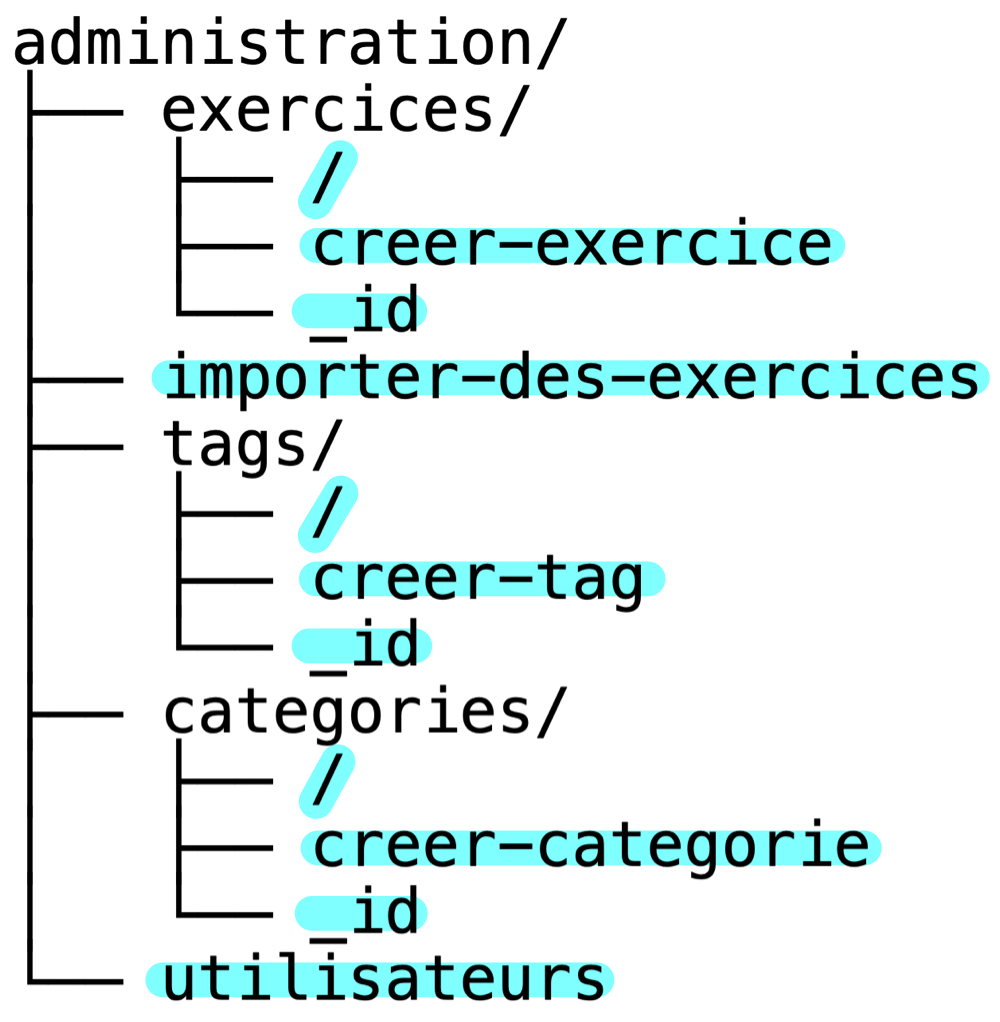
\includegraphics[width=\textwidth,height=0.25\textheight,keepaspectratio]{images/client/administration.jpeg}
    \centering
    \caption[SourceCode : partie administration (URL)]{Partie administration (URL)}
\end{figure}

\subsubsection{La gestion des \glspl{resinfo}}
\label{section:resInfoAdmin}

La gestion des \glspl{resinfo} fonctionne exactement comme la gestion de ses propres \glspl{resinfo}. Reportez-vous donc à la section \ref{section:gestionResInfo} pour connaître les fonctionnalités communes aux utilisateurs et aux administrateurs.

L'administrateur possède les fonctionnalités additionnelles suivantes pour la gestion des \glspl{resinfo} :

\subsubsubsection{Export des résultats de recherche}
 
En filtrant les \glspl{resinfo} par \glspl{tag} et/ou par titre de recherche, vous pouvez exporter tous les résultats correspondant à ce filtrage dans un fichier JSON. Le format de ce fichier est décrit sur l'api (\url{https://sourcecodeoer.github.io/sourcecode_api/#operation/ExportExercises}).

\subsubsubsection{Actions supplémentaires} 

Par rapport à un utilisateur classique, vous pouvez changer l'état d'une \gls{resinfo} de manière plus large comme l'archivage ou la validation.

Pour connaître ces états et leur utilité, reportez-vous à la section \ref{section:statutDuneRessource} et la section \ref{section:analyseFonctionnelle} pour l'état d'une \gls{fiche}.

\subsubsubsection{Champ supplémentaire dans le tableau des ressources} 

Le créateur de la \gls{resinfo}. À ce stade du développement, nous ne pouvons pas contacter l'utilisateur directement depuis la plateforme. C'est définitivement une piste que nous allons explorer dans le chapitre \ref{chapter:pourAllerPlusLoin} car nous aurions voulu intégrer un système de tickets complétant la validation par statut d'une ressource.\\

\subsubsection{L'importation de \glspl{resinfo}}

Améliorer le processus de création de \glspl{resinfo} est une de nos principales préoccupations pour \texttt{SourceCode}. Nous avons alors développé une interface prenant en charge l'importation de \glspl{resinfo}.

\begin{figure}[H]
    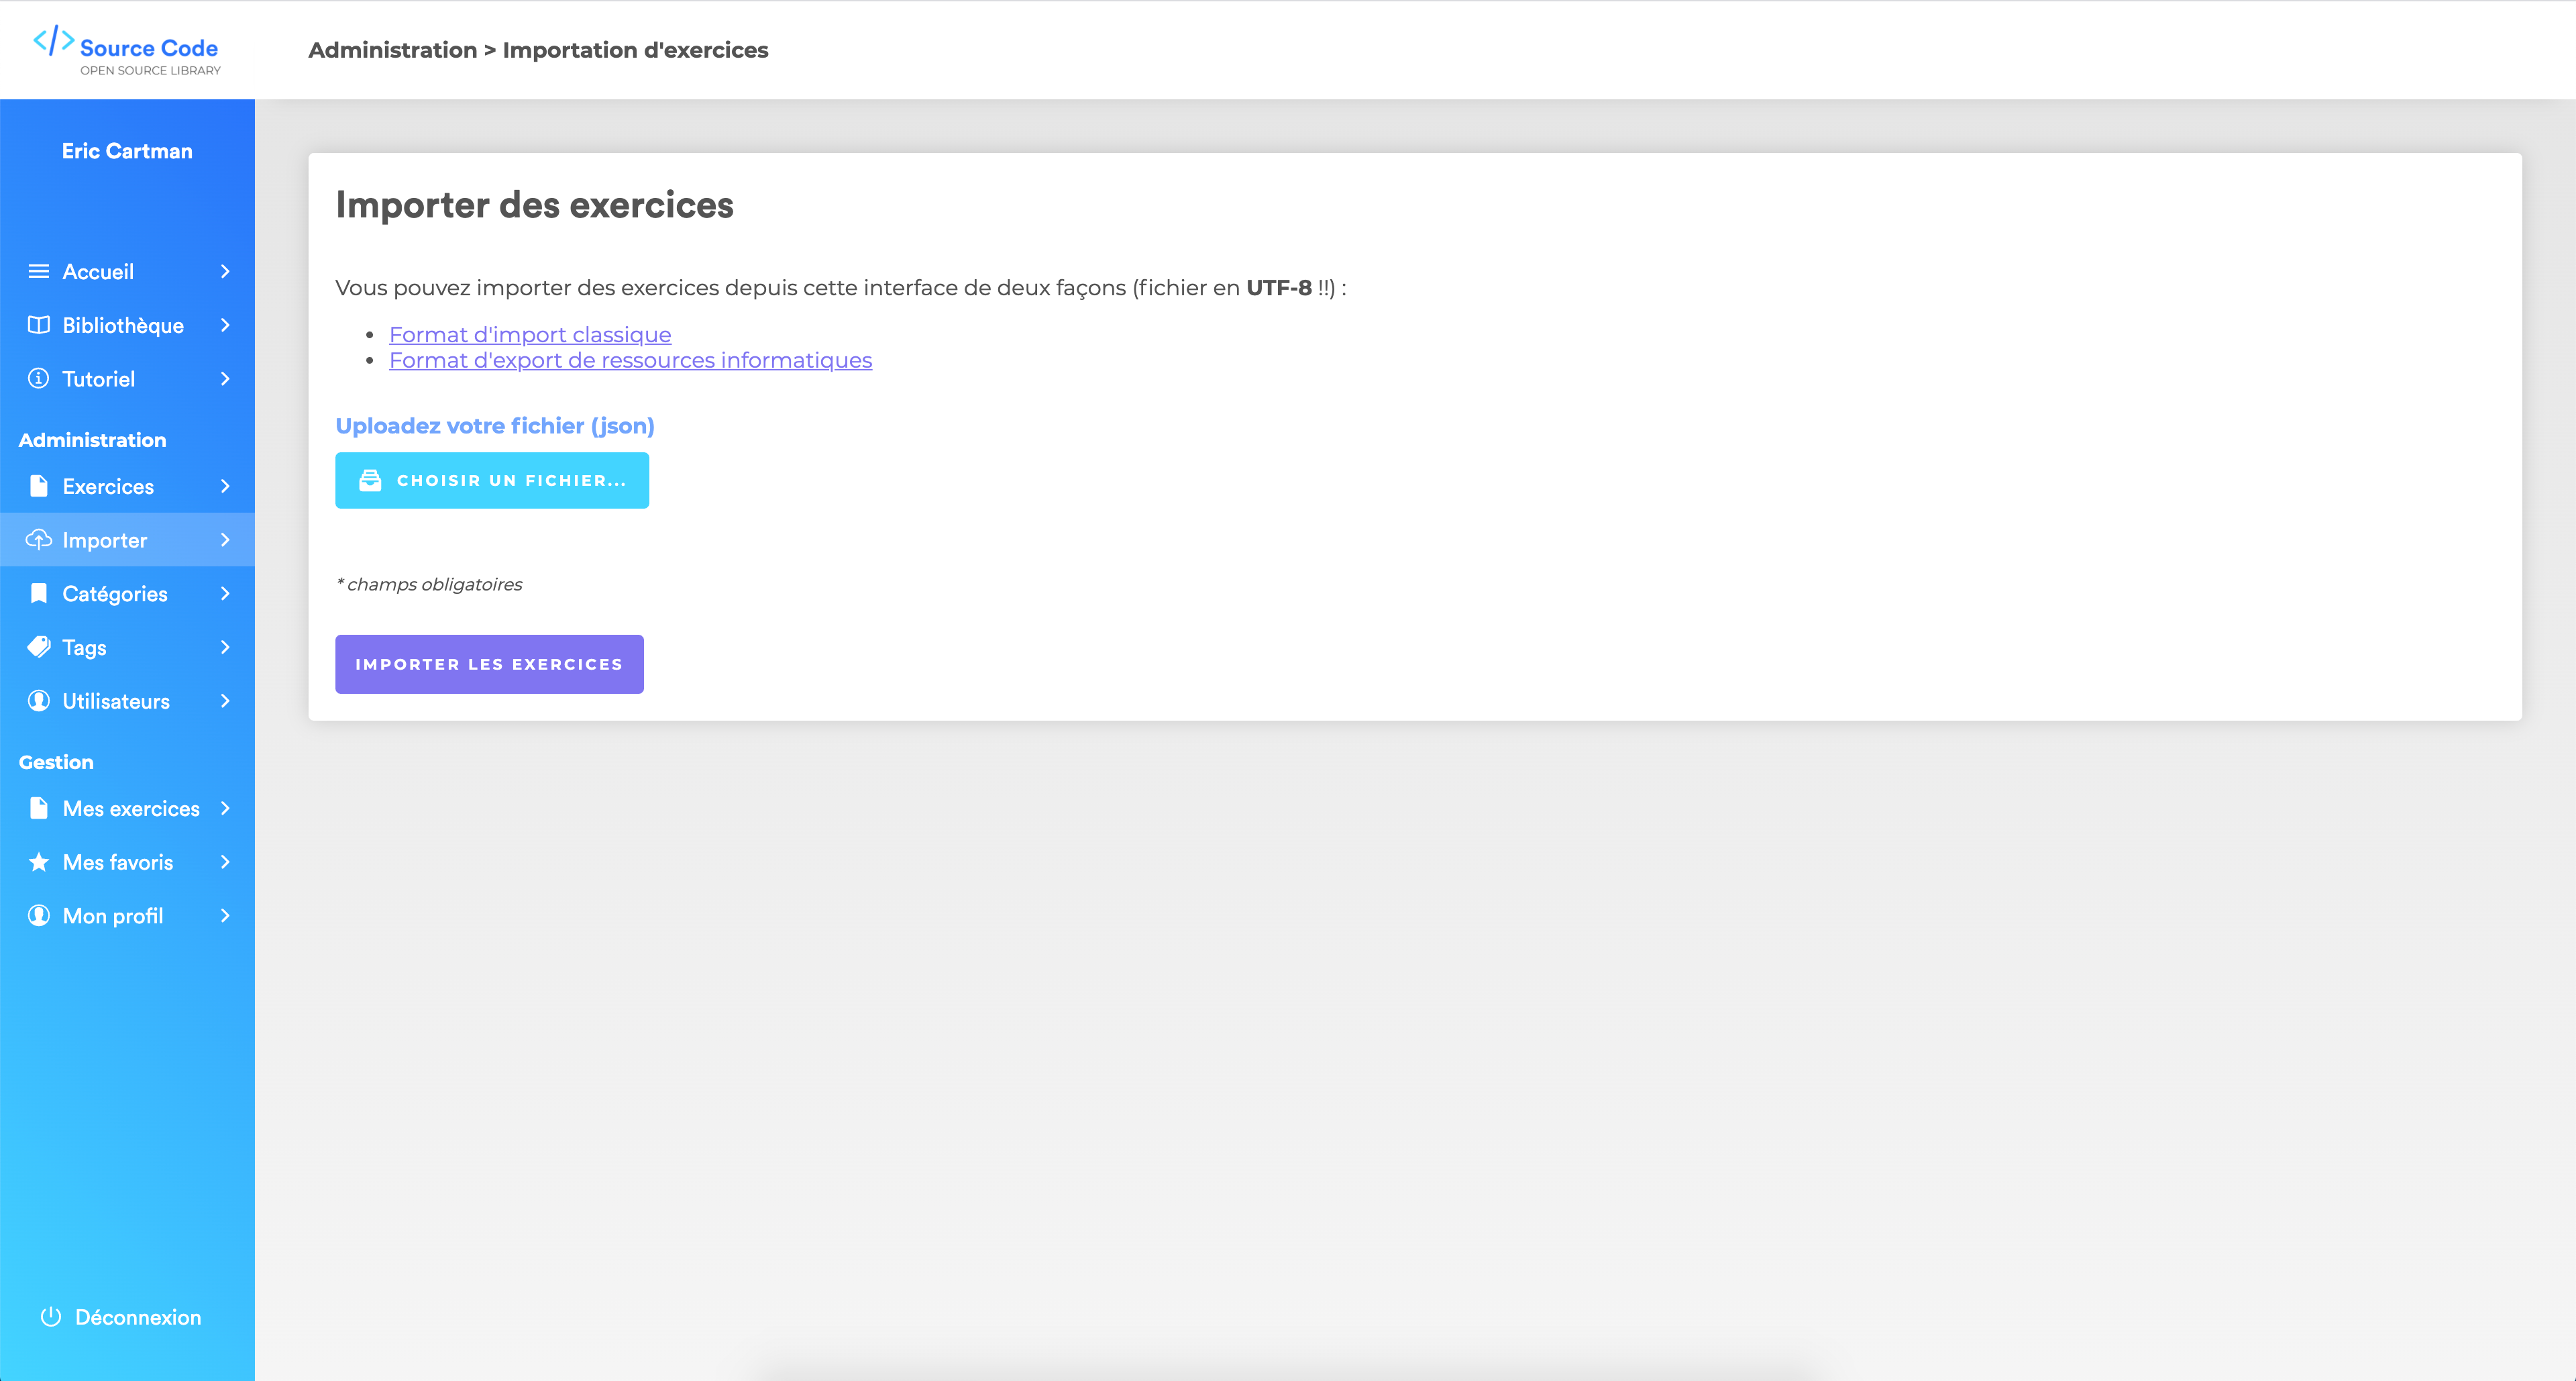
\includegraphics[width=\textwidth,height=\textheight,keepaspectratio]{images/client/import.png}
    \centering
    \caption[SourceCode : importation des \glspl{resinfo}]{Importation des \glspl{resinfo} (importer-des-exercices)}
\end{figure}

Les \glspl{resinfo} doivent être importées avec un fichier JSON respectant un des deux formats que nous vous invitons à consulter :

\begin{itemize}
    \item Format d'import classique (\url{https://sourcecodeoer.github.io/sourcecode_api/#operation/createMultipleExercises})
    \item Format d'export de ressources informatiques (\url{https://sourcecodeoer.github.io/sourcecode_api/#operation/ExportExercises})
\end{itemize}

Nous avons choisi de réserver cette fonctionnalité aux (super-)administrateurs, car il pourrait y avoir des dérives au niveau des simples utilisateurs (attaques DDOS sur l'\gls{api}, ...). À ce propos, la section \textbf{???} de la partie backend explique de manière plus concise notre choix concernant les privilèges de cette fonctionnalité.

\subsubsection{La gestion des \glspl{tag}}
\label{section:tagAdmin}

Les (super-)administrateurs ont la possibilité de gérer les \glspl{tag} présents sur la plateforme. Ils peuvent donc créer des \glspl{tag}, les modifier et changer le statut de ceux-ci.\\

L'interface de gestion prévue à cet effet est semblable à celle de la gestion des ressources informatiques (voir \ref{section:resInfoAdmin}), mis à part que les filtres se limitent aux \glspl{tagCat} et au statut des \glspl{tag}.

\subsubsubsection{Statuts des \glspl{tag}}

De la même manière que pour les \glspl{resinfo}, nous proposons un système de statuts pour donner une indication sur l'état d'un \gls{tag} (la figure \ref{pic:stateDiagramForTags} représente ces états sur un diagramme UML). Nous voulons que le système de \glspl{tag} soit évolutif et flexible. Nous laissons donc les utilisateurs de la plateforme ajouter leurs \glspl{resinfo}, mais aussi des propositions de \glspl{tag} afin d'agrandir le vocabulaire de \texttt{SourceCode}.\\

Cela passe bien évidemment par la validation des administrateurs, qui agissent de concert pour offrir un vocabulaire contrôlé aux utilisateurs, évoluant ainsi en fonction des besoins (voir analyse bibliographique en annexe \ref{annexe:AnalyseBiblio}).

Voici la liste des différents statuts que peut prendre un \gls{tag} :

\begin{itemize}
    \item 
\includegraphics[valign=b,height=1.4\fontcharht\font`X]{images/client/pending.png} \textbf{En attente de validation}
    \begin{itemize}
        \item Le \gls{tag} est mis en attente pour révision. Un administrateur se chargera de le valider ultérieurement.
    \end{itemize}
    \item 
\includegraphics[valign=b,height=1.4\fontcharht\font`X]{images/client/validated.png} \textbf{Valide}
    \begin{itemize}
        \item Lorsque le \gls{tag} est accepté par l'administration, il est alors validé et disponible publiquement dans la bibliothèque.
    \end{itemize} 
    \item 
\includegraphics[valign=b,height=1.4\fontcharht\font`X]{images/client/not-validated.png} \textbf{Invalide}
    \begin{itemize}
        \item Lorsque le \gls{tag} n'est pas considéré comme valide (faute de frappe, doublons, incohérences), l'administrateur se réserve le droit d'invalider le tag. Il pourra néanmoins être modifié (par un admin) pour le revalider plus tard.
    \end{itemize}
    \item 
\includegraphics[valign=b,height=1.4\fontcharht\font`X]{images/client/archive.png} \textbf{Archive}
    \begin{itemize}
        \item Quand un \gls{tag} n'est plus d'utilité ou est remplacé par un autre.
    \end{itemize}
\end{itemize}

La suppression physique d'un \gls{tag} est possible, mais elle est réservée au super-administrateur car c'est une opération irréversible. C'est pour cela que l'existence d'un statut "obsolète" a été mis en place : garder une trace sur l'évolution du vocabulaire de \texttt{SourceCode}.

\subsubsubsection{Création/modification de \glspl{tag}}

Le formulaire de création/modification d'un \gls{tag} requiert les éléments suivants pour être publié :

\begin{itemize}
    \item \textbf{Un nom} : le nom du \gls{tag}
    \item \textbf{Une catégorie} : la \gls{tagCat} auquel il se rapporte
\end{itemize}

La publication du \gls{tag} s'effectue en choisissant un des 4 statuts expliqués précédemment.


\subsubsection{La gestion des \glspl{tagCat}}

La gestion des \glspl{tagCat} se limite uniquement à la modification du titre ou à la création d'une nouvelle catégorie. La suppression est réservée au super-administrateur car elle implique la suppresion de tous les \glspl{tag} qui se rapportent à cette catégorie (opération dangereuse et irréversible).

\subsubsection{La gestion des utilisateurs}

Les administrateurs ont accès à la liste de tout type d'utilisateur ayant un compte enregistré sur \texttt{SourceCode}. Ils peuvent accéder aux informations suivantes :

\begin{itemize}
    \item Le nom de l'utilisateur
    \item L'email de l'utilisateur
    \item Le rôle de l'utilisateur (simple utilisateur, administrateur, super-administrateur)
\end{itemize}

Depuis cette interface, il est possible de modifier le rôle de certains utilisateurs pour les promouvoir ou les destituer d'un rôle. Cette fonctionnalité est uniquement disponible pour le super-administrateur car lui seul devrait garder le contrôle permanent de l'application pour éviter tout débordement.
